% 変分推論による確率的ボラティリティモデルの高速ベイズ推定（社内限定）
% コンパイル：LuaLaTeX（Overleaf では Menu → Compiler → LuaLaTeX。latexmkrc でも指定済み）
% 参考文献：biblatex + biber（Overleaf は自動で biber を実行する）
\documentclass[a4paper,11pt]{ltjsarticle}

\usepackage[margin=25mm]{geometry}
\usepackage{amsmath,amssymb,bm}
\usepackage{graphicx}
\usepackage{booktabs}
\usepackage{xcolor}
\usepackage{enumitem}
\usepackage[
  backend=biber,
  style=authoryear,
  maxcitenames=2,
  maxbibnames=10,
  giveninits=true,
  uniquename=false,
  uniquelist=false,
  dashed=false,
]{biblatex}
\addbibresource{references.bib}
\usepackage[hidelinks]{hyperref}
\usepackage[nameinlink,noabbrev]{cleveref}

% ---------------------------------------------------------------- 相互参照の書式（日本語）
% \jacref{型}{前置}{後置}：単独「第5章」、複数「第5章・第7章」、範囲「第5章〜第8章」
\newcommand{\jacref}[3]{%
  \crefformat{#1}{##2#2##1#3##3}%
  \Crefformat{#1}{##2#2##1#3##3}%
  \crefmultiformat{#1}{##2#2##1#3##3}{・##2#2##1#3##3}{・##2#2##1#3##3}{・##2#2##1#3##3}%
  \Crefmultiformat{#1}{##2#2##1#3##3}{・##2#2##1#3##3}{・##2#2##1#3##3}{・##2#2##1#3##3}%
  \crefrangeformat{#1}{##3#2##1#3##4〜##5#2##2#3##6}%
  \Crefrangeformat{#1}{##3#2##1#3##4〜##5#2##2#3##6}%
  \crefrangemultiformat{#1}{##3#2##1#3##4〜##5#2##2#3##6}{・##3#2##1#3##4〜##5#2##2#3##6}{・##3#2##1#3##4〜##5#2##2#3##6}{・##3#2##1#3##4〜##5#2##2#3##6}%
  \Crefrangemultiformat{#1}{##3#2##1#3##4〜##5#2##2#3##6}{・##3#2##1#3##4〜##5#2##2#3##6}{・##3#2##1#3##4〜##5#2##2#3##6}{・##3#2##1#3##4〜##5#2##2#3##6}%
}
\jacref{section}{第}{章}
\jacref{subsection}{}{節}
\jacref{subsubsection}{}{節}
\jacref{appendix}{付録}{}
\jacref{subappendix}{付録}{}
\jacref{figure}{図}{}
\jacref{table}{表}{}
\jacref{equation}{式(}{)}

% ---------------------------------------------------------------- 記法
\newcommand{\E}{\mathbb{E}}
\newcommand{\KL}{\mathrm{KL}}
\newcommand{\ELBO}{\mathrm{ELBO}}
\newcommand{\Normal}{\mathcal{N}}
\newcommand{\diag}{\mathrm{diag}}
\newcommand{\code}[1]{\texttt{#1}}

\title{変分推論による確率的ボラティリティモデルの高速ベイズ推定\\[0.3em]
  \large ―― MCMC との比較と実務システムへの適用 ――}
\author{（著者名）}
\date{2026 年 11 月（草稿・社内限定）}

\begin{document}

\maketitle

\begin{abstract}
（執筆予定）
\end{abstract}

% 1 章：はじめに
% 数値の出典：memo/09_results_synthetic.md（S1〜S4）、memo/10_results_empirical.md（R1〜R4）、docs/tables/*.tex
\section{はじめに}\label{sec:intro}

\subsection{背景：ボラティリティ推定の実務上の位置付け}\label{sec:intro-background}

金融機関の業務システムにおいて、資産価格の変動の大きさ、すなわちボラティリティは、最も基本的で、かつ最も頻繁に使われる入力の一つである。
ボラティリティの推定値を入力として使う業務は多い。主なものを挙げる。

\begin{itemize}
  \item \textbf{市場リスク管理}：
    バリュー・アット・リスク（VaR）や期待ショートフォール（ES）は、保有ポートフォリオの損益分布の裾を表す指標であり、その計算はリターンの条件付き分布、とりわけその散らばりの推定から始まる。
    バーゼル銀行監督委員会による市場リスクの最低所要自己資本の枠組み \parencite{bcbs2019} では、内部モデル方式で使うリスク指標が 99\% VaR から 97.5\% ES に改められ、損益分布の裾をより重視する方向に進んでいる。
    裾の推定は、ボラティリティの推定の質に直接左右される。
  \item \textbf{デリバティブの評価とヘッジ}：
    オプションの価格やヘッジ比率（デルタなど）は将来のボラティリティに依存する。
    市場で観測されるインプライド・ボラティリティと、過去のリターンから推定したボラティリティを比べることは、値付けの妥当性の確認やトレーディングの判断材料になる。
  \item \textbf{ポートフォリオの構築と運用}：
    ボラティリティ・ターゲティング（ボラティリティが上がったらポジションを落とす）、リスクパリティ（各資産のリスク寄与を揃える）、個別銘柄のポジションサイズの決定などでは、ボラティリティの推定値がそのまま売買の量を決める。
  \item \textbf{証拠金・担保・与信の管理}：
    清算機関や取引相手に差し入れる証拠金、担保の掛け目、市場性与信の枠などは、価格変動の大きさに応じて決まる。
  \item \textbf{モニタリングとアラート}：
    相場の急変を検知し、リスク管理部門やフロントに通知する仕組みでも、「いまのボラティリティが平常時と比べてどの程度高いか」が判断の基準になる。
\end{itemize}

ボラティリティが時間を通じて一定ではないことは、古くからよく知られている。
大きな価格変動の後には大きな変動が続き、穏やかな時期は穏やかな時期が続く（ボラティリティ・クラスタリング）。
また、日次リターンの分布は正規分布よりも裾が厚い。
本稿で使う実データ（日経平均株価と TOPIX に連動する ETF の 2024 年 9 月から 2026 年 8 月までの日次リターン、\cref{sec:empirical}）でも、
年率換算のボラティリティ（事後平均）は期間の中央値で 16〜21\% 程度であるのに対し、
2025 年 4 月の米国の関税政策をきっかけとした急落・急反発の局面では、数営業日のうちに 57〜61\% まで跳ね上がった。
こうした急変に素早く追随しつつ、平常時には過剰に反応しないことが、ボラティリティの推定に求められる。

システムを作る立場から見ると、ボラティリティの推定は一度だけ行う分析ではなく、
\textbf{多数の銘柄について、毎営業日、決められた時刻までに}繰り返し実行されるバッチ処理である。
例えば、夜間バッチで数百〜数千の銘柄のボラティリティを推定し、その結果を翌朝の寄り付き前までにリスク計算やレポートに渡す、といった形になる。
推定結果は下流のリスク計算・規制報告・顧客向けの帳票などに流れるため、推定処理には次のような要件が課される。

\begin{itemize}
  \item \textbf{処理時間が予測できること}：バッチの締め切りに間に合うかどうかを事前に見積もれること。銘柄数やデータ長が増えたときの伸び方が分かっていること。
  \item \textbf{失敗しにくく、失敗を検知できること}：推定がうまくいかなかったときに、それを自動で検知し、再実行やフォールバックができること。
  \item \textbf{結果が再現できること}：同じ入力と設定からは同じ結果が得られ、後から監査や検証ができること。
  \item \textbf{説明できること}：推定値がなぜその値になったのかを、リスク管理部門・監査・監督当局に説明できること。とくに、リスクを小さく見積もる方向の偏りは強く問題視される。
\end{itemize}

これらの要件は、どのモデルを使うかだけでなく、\textbf{そのモデルをどのような計算方法で推定するか}の選択を大きく左右する。
これが本稿の問題意識の出発点である。

\subsection{GARCH 型モデルと確率的ボラティリティモデル}\label{sec:intro-models}

時間変動するボラティリティを表す統計モデルには、大きく二つの系統がある。

一つは GARCH 型のモデルである。代表的な GARCH(1,1) モデル \parencite{bollerslev1986} では、日次リターン $y_t$ の条件付き分散 $\sigma_t^2$ を
\[
  \sigma_t^2 = \omega + \alpha\, y_{t-1}^2 + \beta\, \sigma_{t-1}^2
\]
と、前日のリターンの二乗と前日の条件付き分散の線形結合で表す。
条件付き分散は過去の観測から\textbf{決定論的に}決まるので、尤度は各日の条件付き密度の積として逐次的に計算でき、最尤法で容易に推定できる。
推定は 1 銘柄あたりミリ秒単位で終わり、解釈もしやすいため、GARCH 型モデルは実務の標準になっている。
本稿でも、実データでの予測性能の比較対象として GARCH(1,1) を使う（\cref{sec:empirical}）。

もう一つが、本稿で扱う\textbf{確率的ボラティリティ（stochastic volatility, SV）モデル} \parencite{taylor1986} である。
基本的な SV モデルは、対数ボラティリティ $h_t$ を観測されない状態変数として
\[
  y_t = \exp(h_t/2)\, \varepsilon_t, \qquad
  h_{t+1} = \mu + \phi\,(h_t - \mu) + \sigma\, \eta_t, \qquad
  \varepsilon_t,\ \eta_t \sim \Normal(0, 1)
\]
と表す（詳しくは\cref{sec:model}）。
$\mu$ は対数ボラティリティの長期的な水準、$\phi$ はその持続性、$\sigma$ はボラティリティ自体の変動の大きさを表す。
GARCH との本質的な違いは、ボラティリティが観測 $y_t$ とは別の固有のショック $\eta_t$ を持つ点にある。
ボラティリティは過去のリターンから決まるのではなく、それ自体が確率的に動く隠れた過程であり、リターンはその過程の「ノイズを含んだ観測」とみなされる。

SV モデルには、実務の観点からもいくつかの利点がある。

\begin{itemize}
  \item \textbf{解釈が自然である}：
    市場に到着する情報の量が日々確率的に変動し、それに応じて価格変動の大きさが変わる、という見方（混合分布仮説、\cite{clark1973}）を素直にモデル化したものと解釈できる。
    また、オプション評価で使われる連続時間の確率ボラティリティモデルを離散時間で表したものとも見なせる。
  \item \textbf{ボラティリティ自体の不確実性を表せる}：
    ベイズ推定では、パラメータ $(\mu,\phi,\sigma)$ だけでなく、各日の対数ボラティリティ $h_t$ についても事後分布が得られる。
    例えば「今日のボラティリティは 25\% である」という点推定だけでなく、「95\% の確からしさで 20〜32\% の範囲にある」という区間として示せることは、リスク管理部門や運用担当者との対話で有用である。
  \item \textbf{拡張が自然である}：
    株価が下落するとボラティリティが上がる傾向（レバレッジ効果）は $\varepsilon_t$ と $\eta_t$ の相関として \parencite{omori2007}、
    ボラティリティの変動だけでは説明しきれない裾の厚さは $\varepsilon_t$ を $t$ 分布にすることで、それぞれ同じ枠組みの中で表せる。
    本稿ではこの二つの拡張も扱う。
  \item \textbf{当てはまりと予測の良さ}：
    SV モデルは ARCH 型モデルと比べて遜色のない、あるいはより良い当てはまりを示すことが報告されている \parencite{kim1998}。
    本稿の実データ分析でも、1 期先の予測分布の良さを測る対数予測スコアで、SV モデルが GARCH(1,1) を上回った（差は小さく、統計的に有意だったのは 2 銘柄のうち 1 銘柄。\cref{sec:empirical}）。
\end{itemize}

一方で、SV モデルには推定上の大きな難しさがある。
パラメータ $\theta = (\mu,\phi,\sigma)$ の尤度は、観測されない $h_1,\dots,h_T$ をすべて積分消去した
\[
  p(y_{1:T} \mid \theta) = \int \prod_{t=1}^{T} p(y_t \mid h_t)\; p(h_{1:T} \mid \theta)\; dh_{1:T}
\]
で与えられる。これは $T$ 次元（日次データ 2 年分なら約 500 次元、10 年分なら約 2,500 次元）の積分であり、閉じた形では計算できない。
GARCH 型モデルでは条件付き分散が観測から決まるためこの積分が現れず、ここが両者の計算コストの違いの根源である。
SV モデルの推定では、この高次元の積分をどう扱うかが常に中心的な問題になる。

\subsection{従来の推定法とシステム運用上の課題}\label{sec:intro-mcmc}

SV モデルの推定法は、これまで数多く提案されてきた。
初期の代表的な方法は、$\log y_t^2 = h_t + \log \varepsilon_t^2$ という変形により観測方程式を線形にし、$\log \varepsilon_t^2$ の分布を正規分布で近似したうえでカルマンフィルタを使う疑似最尤法（QML）である \parencite{harvey1994}。
計算は速いが、$\log \varepsilon_t^2$ の分布（裾が非対称な $\log \chi^2_1$ 分布）を正規分布で置き換えるため、推定の効率が落ちる。

その後、\textbf{マルコフ連鎖モンテカルロ法（MCMC）}によるベイズ推定が SV モデルの標準的な推定法になった。
\textcite{jacquier1994} は、$h_t$ を一つずつ更新する MCMC で、パラメータと潜在ボラティリティの事後分布を同時に求める方法を示した。
\textcite{kim1998} は、$\log \varepsilon_t^2$ の分布を正規分布の混合で精度よく近似することで、$h_{1:T}$ 全体をカルマンフィルタ・スムーザーを使って一度にサンプリングする効率的な方法を提案した。
\textcite{omori2007} はこれをレバレッジ効果のあるモデルに拡張し、
\textcite{chan2009} は、状態変数の事後分布の精度行列（共分散行列の逆行列）が帯行列になることを使って、状態を $O(T)$ の計算量で一括してサンプリングする方法を示した。
\textcite{kastner2014} は、中心化・非中心化という二つのパラメータ化を交互に使う ASIS という手法で、とくに $\sigma$ の混合（サンプルの自己相関の小ささ）を大きく改善している。
日本語の解説としては \textcite{watanabe2000} がある。

近年は、モデルを確率的プログラミング言語で書けば勾配情報を使って自動的にサンプリングできる、汎用の MCMC 手法も普及した。
その代表が、ハミルトニアン・モンテカルロ法の歩幅や軌道の長さを自動で調整する No-U-Turn Sampler（NUTS）\parencite{hoffman2014} であり、Stan や NumPyro \parencite{phan2019} などのライブラリで使える。
本稿では、NumPyro の NUTS を十分に長く回した結果を、事後分布の「正解」として扱う。

MCMC は、反復を十分に長くとれば事後分布を正確に表すサンプルが得られる（漸近的に正確な）方法であり、研究の場では SV 推定の標準である。
しかし、前節で述べたシステムの要件に照らすと、次のような課題がある。

\begin{enumerate}[label=(\arabic*)]
  \item \textbf{計算時間が長く、しかも事前に読みにくい}：
    MCMC のサンプルは互いに相関しているため、事後分布を十分な精度で表すには、得たいサンプル数の何倍もの反復が必要になる。
    その倍率はモデル・データ・パラメータ化によって大きく変わり、事前には分からない。
    本稿の計算時間の実験（\cref{sec:synthetic}）では、系列長 $T=10{,}000$ の SV モデルに NUTS を（ウォームアップ・サンプリング各 1,000 反復、4 チェーンで）適用すると 548 秒かかり、
    しかもパラメータの有効サンプルサイズ（ESS：自己相関を考慮した実質的なサンプル数）は最小で 14 しかなかった。
  \item \textbf{収束の判定と、判定に落ちたときの扱いが難しい}：
    MCMC の結果を使ってよいかは、複数チェーン間の一致度 $\hat R$、ESS、発散の有無などで判定する。
    判定自体は自動化できるが、基準を満たさなかったときに反復を延長するのか、パラメータ化を変えて再実行するのか、といった運用の設計が必要になる。
    本稿の実験でも、標準的な設定（ウォームアップ・サンプリング各 2,000 反復、4 チェーン）では、
    合成データの 200 回の推定のうち 156 回、実データの 32 銘柄のうち 11 銘柄で、パラメータの $\hat R$ が目安の 1.05 を超えた（\cref{sec:synthetic,sec:system}）。
    SV モデルの MCMC で $\sigma$ の混合が悪いことはよく知られた問題であり \parencite{kastner2014}、汎用の NUTS でもそれは解消されない。
  \item \textbf{銘柄数・再推定の頻度とともに計算量が積み上がる}：
    実データの 32 銘柄（各 485 日）を NUTS で 1 銘柄ずつ推定すると、合計で 293 秒かかった（\cref{sec:system}）。
    実務では、これが銘柄数（数百〜数千）、モデルの種類、毎営業日の再推定の分だけ掛け算で増える。
    前日の結果を初期値に使うことはできるが、MCMC ではウォームアップ（歩幅などの適応）とサンプリングそのものは毎回必要であり、計算量はあまり減らない。
\end{enumerate}

\subsection{変分推論という選択肢とその落とし穴}\label{sec:intro-vi}

こうした背景から、本稿では\textbf{変分推論（variational inference, VI）}に注目する \parencite{blei2017}。
VI は、事後分布 $p(\theta, h_{1:T} \mid y_{1:T})$ を、計算しやすい分布の族 $\mathcal{Q}$（例えば多変量正規分布の族）の中で最も近い分布 $q^\ast$ で近似する方法である。
近さはカルバック・ライブラー情報量 $\KL(q \,\|\, p)$ で測り、それを最小化する代わりに、等価な目的関数である証拠下界（ELBO）を最大化する（\cref{sec:inference}）。
つまり VI は、\textbf{積分（サンプリング）の問題を最適化の問題に置き換える}。
再パラメータ化による勾配の推定 \parencite{kingma2014} と自動微分を組み合わせると、モデルの対数密度を書くだけで確率的勾配法により最適化できる。
これを、制約のあるパラメータの変換まで含めて自動化したものが自動微分変分推論（ADVI）\parencite{kucukelbir2017} である。

システムの観点から見ると、VI には次のような利点がある。

\begin{itemize}
  \item \textbf{速い}：数千ステップの勾配法で済み、MCMC より桁違いに短い時間で事後分布の近似が得られる。
  \item \textbf{処理時間が予測しやすい}：計算量は「ステップ数 × 1 ステップのコスト」で決まり、ステップ数は設定で固定できる。収束の判定も、目的関数（ELBO）の推移という一つの数値列を見ればよい。
  \item \textbf{前日の結果を再利用できる}：最適化なので、前日の最適解から再開（warm start）すれば、少ないステップで今日の解に到達できる。
  \item \textbf{並列化・一括処理と相性が良い}：銘柄ごとの最適化は互いに独立であり、そのまま複数の計算資源に振り分けられる。
  \item \textbf{結果を固定長の数値として保存できる}：推定結果は変分分布のパラメータ（数千個の数値）として保存でき、そこから必要なときに必要な数だけサンプルを生成できる。乱数のシードを固定すれば再現も容易である。
\end{itemize}

ただし、VI には重要な落とし穴がある。
第一に、VI は近似であり、得られる分布の精度の上限は、あらかじめ選んだ族 $\mathcal{Q}$ の表現力で決まる。反復を増やしても、族の外にある真の事後分布には近づかない。
第二に、VI が最小化する $\KL(q \,\|\, p)$ は非対称な量であり、真の事後分布 $p$ の確率が小さいところに $q$ が確率を置くことを強く罰する。
その結果、$q$ は $p$ の裾を切り捨てる傾向があり、\textbf{事後分布の分散（不確実性）を過小評価しやすい} \parencite{blei2017}。
リスク管理の文脈では、これは「リスクを実際より小さく見せる」方向の偏りであり、前節で述べた説明責任の観点から最も避けたい性質である。

とりわけ問題になるのが、最も単純で広く使われる\textbf{平均場近似}（すべての変数を互いに独立とみなす族）である。
SV モデルでは、対数ボラティリティ $h_t$ が $\phi \approx 0.95$〜$0.99$ という強い持続性を持ち、事後分布でも隣り合う日の $h_t$ どうしが強く相関する。
平均場近似はこの相関をまったく表せない。
本稿の実験では、平均場近似による VI は、真値が 0.97〜0.99 のシナリオで持続性 $\phi$ の推定値を 0.03〜0.3 程度まで崩してしまい、
「分散を過小評価する」という教科書的な問題以前に、\textbf{パラメータの点推定そのものが大きく偏る}ことが分かった（\cref{sec:synthetic}）。
一方で、表現力を上げるために変数間の相関をすべて許すフルランクの正規分布（変分パラメータは約 50 万個）を使っても、
最適化が難しくなり、真値 $\phi = 0.99$、$T = 1{,}000$ のデータに 230 秒かけても $\phi = 0.24$ にとどまった。
\textbf{パラメータを増やせばよいわけではなく、モデルの構造に合った族を選ぶことが重要}なのである。

したがって、SV モデルに VI を使えるかどうかは、
「SV の事後分布の構造を正しく捉えつつ、VI の速さと運用上の利点を保てる変分族を設計できるか」にかかっている。

\subsection{関連研究と本稿の位置付け}\label{sec:intro-related}

時系列の状態空間モデルに対する VI では、状態変数の時間方向の依存を変分族に組み込む研究が進んできた。
\textcite{archer2015} は、時間方向にブロック三重対角の精度行列を持つ正規分布を変分族とし、カルマンフィルタ・スムーザーと同じ直観で、非線形な状態空間モデルにも使える汎用の VI を構成した。
\textcite{tan2018} は、精度行列のコレスキー因子にモデルの条件付き独立性に応じた疎な構造を課した正規分布による変分近似を提案し、状態空間モデルに適用している。
これらは、MCMC の側で \textcite{chan2009} が使った「帯行列の精度行列による $O(T)$ の計算」と同じ構造を、変分族の側で利用するものである。

さらに、パラメータ（大域変数）と状態（局所変数）の事後的な依存を変分族に取り入れる研究もある。
\textcite{tan2020} は、階層モデルでは分散などの大域パラメータが局所潜在変数の事後分布の尺度を決めることに着目し、局所変数の変分分布を大域パラメータに条件付けた族を提案して、一般化線形混合モデルや状態空間モデルに適用した。
\textcite{loaizamaya2022} は、パラメータには簡潔なパラメトリック近似を使い、潜在変数には（近似ではなく）正確な条件付き事後分布を使う族を提案し、その密度を計算できなくても、条件付き事後分布からサンプリングさえできれば勾配が計算できることを示した。
\textcite{frazier2023} は、状態空間モデルでよく使われる VI の方法を比較し、状態の事後分布を近似しない方法の方が、状態まで近似する方法よりもパラメータの推定が正確であること、
ただし推論の精度の差は短い検証期間では予測精度の小さな差にしかならないことが多い一方、長い検証期間では意味のある差になりうることを報告している。
機械学習の分野では、\textcite{johnson2016} が、状態の事後分布を「事前分布 × ニューラルネットワークが出力する共役な因子（擬似観測）」の形で表す構造化 VI を提案している。

SV モデルそのものに VI を適用した研究としては、
多変量の因子 SV モデルに対する高速な変分ベイズ法と、新しい観測が来たときの逐次的な変分更新を提案した \textcite{gunawan2021}、
多数の変数を持つベイズ VAR の SV 部分について、対数ボラティリティの同時事後分布を大域的に近似する方法を提案した \textcite{chan2022}、
状態の同時事後分布を動的因子モデルで近似する正規分布の変分近似を、Wishart 型の多変量 SV モデルに適用した \textcite{quiroz2023} などがある。

本稿で提案として扱う\textbf{条件付き構造化変分族}（\cref{sec:family}）は、
状態 $h_{1:T}$ の変分分布をパラメータ $\theta$ に条件付け、その形を「AR(1) の事前分布 × 正規分布の擬似観測」とするものである。
これは、上に挙げた考え方、とくに \textcite{tan2020} の条件付きの構造と \textcite{johnson2016} の擬似観測による表現を、一変量の SV モデルに素直に当てはめたものであり、
手法として新しいことを主張するものではない。
本稿の主眼はむしろ、次の三点にある。

\begin{itemize}
  \item 平均場近似から条件付き構造化まで、\textbf{変分族の設計の違いが結果をどれほど変えるか}を、同じ実装・同じ条件のもとで、真値（合成データ）と十分に長い MCMC を基準に定量的に示すこと。
  \item 日本の株式市場の実データ（ETF と個別株）で、事後分布の一致だけでなく、\textbf{VaR の予測性能まで}評価すること。
  \item システムに載せるときの具体的な論点（日次の再推定、多銘柄の並列化、結果の監視、MCMC との使い分け）を、\textbf{実測に基づいて}整理すること。
\end{itemize}

\subsection{本稿の目的と貢献}\label{sec:intro-contrib}

本稿の目的は、SV モデルのベイズ推定を VI で行うことが金融機関向けシステムの実務に使えるかを、\textbf{精度・計算時間・運用性}の三つの観点から評価し、
使えるとすればどのように使うべきかを示すことである。
本稿の貢献は次の四つにまとめられる。

\begin{enumerate}[label=(\roman*)]
  \item \textbf{SV モデルに対する変分族の体系的な比較}（\cref{sec:family,sec:synthetic}）。
    基本 SV・レバレッジ SV・$t$ 誤差 SV の三つのモデルについて、
    平均場、低ランク、フルランク、構造化（パラメータと状態を独立とし、状態は三重対角の精度行列を持つ正規分布）、条件付き構造化の各変分族を、
    真値が分かっている合成データ（5 つのシナリオ × 2 つの系列長 × 各 20 本）と、十分に長く回した NUTS を基準に比較した。
    その結果、平均場・低ランク・フルランクの族はいずれも持続性 $\phi$ の推定が崩れること、
    構造化の族は状態 $h_t$ の推定は良好だが $\sigma$ の不確実性を 1/5〜1/10 に過小評価し、$\sigma$ の 95\% 区間が真値をほとんど含まないことを示した。
  \item \textbf{条件付き構造化変分族の構成と評価}（\cref{sec:family,sec:synthetic}）。
    $q(\theta, h) = q(\theta)\, q(h \mid \theta)$、
    $q(h \mid \theta) \propto p(h \mid \theta) \prod_{t} \Normal(\tilde y_t \mid h_t, \lambda_t^{-1})$
    という族を、SV モデル向けに具体的に構成した（$\tilde y_t$ と $\lambda_t$ が変分パラメータ）。
    $\theta$ を固定すると $q(h \mid \theta)$ の精度行列は三重対角になり、サンプリングも密度の計算も $O(T)$ で済む。
    また、この族は中心化・非中心化というパラメータ化の選び方に依存しない。レバレッジ SV への拡張も示した。
    持続性の高いシナリオ（$\phi = 0.99$、$T = 1{,}000$）で、事後平均は NUTS とほぼ一致し（$\phi$：0.983 対 0.983、$\sigma$：0.123 対 0.126）、
    $h_t$ の事後標準偏差も NUTS の 0.98 倍と、不確実性の大きさまで再現できた。
    計算時間は $T = 10{,}000$ で約 11 秒であり、NUTS（548 秒）の約 50 倍速い。
  \item \textbf{日本の株式市場の実データでの評価}（\cref{sec:empirical}）。
    J-Quants API の無料プランで取得した、日経平均株価・TOPIX に連動する ETF（1321・1306）と TOPIX Core30 構成銘柄の日次リターン（485 営業日）を使った。
    全期間の推定では、提案手法の事後分布は NUTS とほぼ一致した（例：1321 の $\phi$ は 0.898 対 0.889）。
    250 日の窓を 1 日ずつずらしながら毎日推定し直す VaR のバックテスト（検証 235 日）では、
    提案手法による SV モデルの 5\% VaR の超過率は 6.4〜6.8\% で、Kupiec の検定・Christoffersen の検定のいずれでも棄却されず、
    対数予測スコアは GARCH(1,1)（正規誤差・$t$ 誤差のいずれ）よりも良かった（ただし差は 1 日あたり 0.03 nats 以下と小さく、Diebold–Mariano 検定で有意だったのは 1306 だけである）。
    一方、平均場近似では 1321 の 5\% VaR の超過率が 8.1\% となり、有意水準 5\% の検定で棄却された。
  \item \textbf{システム実装の観点からの知見}（\cref{sec:system}）。
    前日の変分パラメータを 1 日ずらして初期値にする warm start により、毎日の再推定は 1 銘柄 1 日あたり 0.10 秒（毎回ゼロから推定する場合の約 1/5）になり、VaR への影響は中央値で 0.02〜0.03\% ポイントと無視できる大きさだった。
    32 銘柄の一括推定は、NUTS の逐次実行で 293 秒、提案手法の逐次実行で 50 秒、8 つの CPU デバイスへの並列実行で 15 秒（NUTS の約 19 倍速い）だった。
    また、銘柄の方向に計算をベクトル化（\code{jax.vmap}）すると 68 秒と、逐次実行よりかえって遅くなることを確認した。
    「ベクトル化すれば速くなる」とは限らず、計算の形とハードウェアに合った並列化を選ぶ必要がある。
    これらを踏まえ、日次の運用は warm start の VI で行い、定期的に MCMC で結果を突き合わせる\textbf{ハイブリッド運用}と、その監視の方法を提案する。
\end{enumerate}

同時に、本稿の結果には限界もある。
提案手法は、レバレッジ SV の相関パラメータ $\rho$ を 0 の側に約 25\% 縮めて推定する。
実データでは、$\sigma$ を NUTS より 8\% ほど小さく、その事後標準偏差も NUTS の約 0.85 倍と、不確実性をやや小さく見積もる傾向が見られた。
VI の当てはまりを自動で診断する指標として提案されている PSIS の $\hat k$ は、手法の良し悪しの順位とはおおむね整合したものの、本稿の問題では提案手法を含むすべての手法で目安の 0.7 を超えた（提案手法でも 0.85）。そのため、「この値を下回れば近似を信頼してよい」という単独の判定基準としては使いにくい。
また、無料プランで取得できるデータは約 2 年分と短く、VaR の検証期間（235 日）では 1\% VaR の検定の検出力が低い。
計算時間はすべて単一の CPU マシン（12 コア）で測ったものであり、GPU での評価は行っていない。
これらの点は\cref{sec:synthetic,sec:empirical,sec:system,sec:conclusion}で詳しく述べる。

\subsection{本稿の構成}\label{sec:intro-outline}

本稿の構成は次のとおりである。

\cref{sec:model}では、基本 SV モデルと、その二つの拡張（レバレッジ効果、$t$ 分布の誤差）を定義し、事前分布を示す。
あわせて、尤度が解析的に書けない理由と、推定上の論点になる中心化・非中心化のパラメータ化を説明する。

\cref{sec:inference}では、ベイズ推定の枠組みと、本稿で「正解」として使う NUTS の概要を述べたうえで、
VI の基礎（KL 情報量と ELBO の関係、再パラメータ化による勾配の推定、ADVI）を、読者が実装の見通しを持てる程度に詳しく説明する。

\cref{sec:family}は本稿の中心であり、SV モデルの事後分布の構造（AR(1) の事前分布の精度行列が三重対角であること）を確認したうえで、
平均場から条件付き構造化までの変分族を定義し、それぞれのサンプリング・エントロピーの計算方法と計算量を比較する。

\cref{sec:synthetic}では、合成データを使って、パラメータの復元精度、NUTS との事後分布の一致度、系列長に対する計算時間の伸び方、設定への感度を評価する。

\cref{sec:empirical}では、J-Quants API で取得した ETF のデータを使って、全期間のボラティリティの推定と、ローリング推定による VaR のバックテストを行い、GARCH(1,1) と比較する。

\cref{sec:system}では、システムに組み込むことを想定して、日次の再推定（warm start）、多銘柄の並列処理、収束の判定と監視、再現性、MCMC との使い分けを、実測の結果に基づいて論じる。

\cref{sec:conclusion}では、結論と今後の課題（多変量 SV、実現ボラティリティの利用、より表現力の高い変分族など）を述べる。

付録には、ELBO の勾配と条件付き構造化変分族の導出（\cref{app:derivation}）、実装の抜粋（\cref{app:code}）、実験設定と感度分析（\cref{app:settings}）、データの取得と前処理（\cref{app:data}）をまとめた。

なお、本稿ではリターンを日次の対数リターンの 100 倍（\% 単位）で表し、標本平均を除いたものを $y_t$ とする。
年率換算のボラティリティは $\sqrt{252}\, \exp(h_t/2)$（\%）で表す。

% 2 章：確率的ボラティリティモデル
% 定義は実装と一致させている：src/sv_vi/logdensity.py（同時密度）、models.py（NumPyro 版）、
% simulate.py（合成データ）、predictive.py（予測分布）。図表は experiments/f1_model_illustration.py が生成。
\section{確率的ボラティリティモデル}\label{sec:model}

本章では、本稿で扱う確率的ボラティリティ（SV）モデルを定義し、その性質を整理する。
\cref{sec:model-data} でデータの単位と記法を定め、\cref{sec:model-basic,sec:model-properties} で基本 SV モデルとその性質（裾の厚さ、ボラティリティ・クラスタリング）を述べる。
\cref{sec:model-leverage,sec:model-t} で二つの拡張（レバレッジ効果、$t$ 分布の誤差）を、\cref{sec:model-prior} で事前分布を示す。
\cref{sec:model-likelihood,sec:model-structure} では、尤度が解析的に書けない理由と、事後分布が持つ構造（三重対角の精度行列）を説明する。
この構造が、\cref{sec:family} で変分族を設計するときの出発点になる。
最後に、推定の実務で重要になるパラメータ化の選択（\cref{sec:model-param}）と、VaR の計算に使う 1 期先の予測分布（\cref{sec:model-predictive}）を述べる。

\subsection{データと記法}\label{sec:model-data}

資産の終値（分割などを調整した価格）を $P_t$ とし、日次の対数リターンを \% 単位で
\[
  r_t = 100\,(\log P_t - \log P_{t-1}), \qquad t = 1, \dots, T
\]
と定義する。本稿のモデルでは、標本平均 $\bar r$ を引いた
\[
  y_t = r_t - \bar r
\]
を観測とする。日次リターンの平均は 0.05\% 程度と、日次の標準偏差（1\% 前後）に比べて十分に小さいので、
平均を定数として事前に除いても推定への影響は小さく、モデルを「散らばりの変動」だけに集中させることができる。
\cref{sec:empirical} のローリング推定では、先読みを避けるため、各時点の推定窓の中だけで平均を計算して除き、翌日のリターンにも同じ平均を使う。

\% 単位を使うのは、数値を扱いやすい範囲に収めるためである。
後で導入する対数ボラティリティ $h_t$ を使うと、日次リターンの条件付き標準偏差は $\exp(h_t/2)$（\%）、
年率換算のボラティリティは $\sqrt{252}\,\exp(h_t/2)$（\%）になる（1 年を 252 営業日とする）。
例えば $h_t = 0$ は日次 1\%、年率約 15.9\% に対応し、$h_t = 1$ なら日次 1.65\%、年率約 26\% である。
生の対数リターン（小数）を使うと $h_t$ は $-9$ 前後の値をとり、同じ事前分布でも意味が変わってしまう。
事前分布の妥当性は単位に依存するので、本稿の事前分布（\cref{sec:model-prior}）は \% 単位を前提に設定している。

記法をまとめておく。$y_{1:T} = (y_1, \dots, y_T)$ のように添字の範囲で列を表し、紛れがなければ単に $y$、$h$ と書く。
$\Normal(m, v)$ は平均 $m$、分散 $v$ の正規分布、$\Normal(x \mid m, v)$ はその密度を $x$ で評価した値である。
モデルの大域パラメータをまとめて $\theta$ と書く。基本 SV モデルでは $\theta = (\mu, \phi, \sigma)$、レバレッジ SV では $\rho$ が、$t$ 誤差の SV では $\nu$ が加わる。

\subsection{基本 SV モデル}\label{sec:model-basic}

基本 SV モデル \parencite{taylor1986,jacquier1994,kim1998} は次の二つの式からなる。
\begin{align}
  y_t &= \exp(h_t/2)\,\varepsilon_t, & \varepsilon_t &\sim \Normal(0, 1), & t &= 1, \dots, T, \label{eq:sv-obs}\\
  h_{t+1} &= \mu + \phi\,(h_t - \mu) + \sigma\,\eta_t, & \eta_t &\sim \Normal(0, 1), & t &= 1, \dots, T-1, \label{eq:sv-state}\\
  h_1 &\sim \Normal\!\left(\mu,\ \frac{\sigma^2}{1-\phi^2}\right). \label{eq:sv-init}
\end{align}
ここで $\varepsilon_t$ と $\eta_s$ はすべての $t, s$ について互いに独立とする（独立でない場合が次節以降のレバレッジ SV である）。

\cref{eq:sv-obs} は\textbf{観測方程式}であり、リターン $y_t$ が、平均 0、分散 $\exp(h_t)$ の正規分布に従うことを表す。
$h_t$ は日次分散の対数（対数ボラティリティ）であり、観測されない\textbf{潜在変数（状態変数）}である。
\cref{eq:sv-state} は\textbf{状態方程式}であり、$h_t$ が平均 $\mu$ のまわりを変動する 1 次の自己回帰過程（AR(1) 過程）に従うことを表す。
\cref{eq:sv-init} は初期値 $h_1$ を AR(1) 過程の定常分布から始めることを意味し、これにより $h_1, h_2, \dots$ はすべて同じ周辺分布 $\Normal(\mu, \sigma^2/(1-\phi^2))$ を持つ。

三つのパラメータの意味は次のとおりである。
\begin{itemize}
  \item $\mu \in \mathbb{R}$：対数ボラティリティの長期的な水準。$h_t$ はショックを受けても、長い目で見ると $\mu$ のまわりに戻ってくる。
    \% 単位のリターンでは、$\mu$ がおよそ $-1$〜$2$（日次 0.6〜2.7\%）の範囲にあることが多い。
  \item $\phi \in (-1, 1)$：対数ボラティリティの持続性。$h_t - \mu$ が 1 日で $\phi$ 倍になって残る。
    株価指数の日次データでは $0.95$〜$0.99$ 程度の値が推定されることが多い。$|\phi| < 1$ は $h_t$ が定常であるための条件である。
  \item $\sigma > 0$：対数ボラティリティそのものの変動の大きさ（ボラティリティのボラティリティ）。
    $\sigma$ が大きいほど、ボラティリティは日々大きく揺れ動く。
\end{itemize}

このモデルは\textbf{状態空間モデル}の一種とみなせる。
$h_{1:T}$ はマルコフ連鎖であり、$h_{t+1}$ の分布は $h_t$ だけで決まる。
また、$h_{1:T}$ をすべて与えると、$y_t$ どうしは互いに独立で、$y_t$ の分布は同じ日の $h_t$ だけで決まる。
したがって同時分布は
\begin{equation}
  p(y_{1:T}, h_{1:T} \mid \theta)
  = \underbrace{p(h_1 \mid \theta) \prod_{t=1}^{T-1} p(h_{t+1} \mid h_t, \theta)}_{p(h_{1:T} \mid \theta)}
    \;\underbrace{\prod_{t=1}^{T} p(y_t \mid h_t)}_{p(y_{1:T} \mid h_{1:T})}
  \label{eq:sv-joint}
\end{equation}
と、「AR(1) 過程の事前分布」と「各日の観測の尤度の積」に分解できる。
各日の観測の対数尤度は
\begin{equation}
  \log p(y_t \mid h_t) = -\frac{1}{2}\log(2\pi) - \frac{h_t}{2} - \frac{y_t^2}{2}\,e^{-h_t}
  \label{eq:sv-loglik}
\end{equation}
である。この分解は、後で事後分布の構造を調べるとき（\cref{sec:model-structure}）にも、変分族を設計するとき（\cref{sec:family}）にも中心的な役割を果たす。

GARCH 型モデルとの違いをもう一度確認しておく。
GARCH(1,1) では、条件付き分散 $\sigma_t^2$ は前日までのリターンから決定論的に計算でき、$y_1, \dots, y_{t-1}$ を知れば $\sigma_t^2$ は確定する。
これに対して SV モデルでは、$h_t$ は過去のリターンを知っても確定せず、確率的なショック $\eta_{t-1}$ の分だけ不確実性が残る。
つまり SV モデルでは、ボラティリティは「観測から計算する量」ではなく「観測から\textbf{推測する}量」であり、その推測の不確実性も含めて扱う必要がある。
この違いが、表現力の高さ（\cref{sec:model-properties}）と、推定の難しさ（\cref{sec:model-likelihood}）の両方の源になっている。

\subsection{基本 SV モデルの性質}\label{sec:model-properties}

基本 SV モデルは単純な形をしているが、金融リターンの代表的な性質である\textbf{裾の厚さ}と\textbf{ボラティリティ・クラスタリング}を再現する。
ここでは、それを定常状態でのモーメントの計算で確認する。
導出は、$h_t$ が正規分布に従うとき $\E[e^{a h_t}] = \exp(a\mu + a^2 s^2/2)$ となること（対数正規分布のモーメント）だけを使う。

\paragraph{定常分布}
$h_t$ の定常分布は $\Normal(\mu, s^2)$ であり、その分散は
\[
  s^2 = \frac{\sigma^2}{1-\phi^2}
\]
である。$s$ は「対数ボラティリティが長期的にどの程度の幅で動くか」を表す。
$\phi$ が 1 に近いと、$\sigma$ が小さくても $s$ は大きくなる。
例えば $\phi = 0.97$、$\sigma = 0.15$ では $s \approx 0.62$ であり、日次の標準偏差 $\exp(h_t/2)$ は定常分布の 95\% の範囲で
$\exp(\pm 1.96 \times 0.62 / 2) \approx 0.55$〜$1.83$ 倍の幅で変動する。

\paragraph{分散と尖度}
$\varepsilon_t$ と $h_t$ が独立であることから、
\[
  \E[y_t^2] = \E[e^{h_t}]\,\E[\varepsilon_t^2] = e^{\mu + s^2/2}, \qquad
  \E[y_t^4] = \E[e^{2h_t}]\,\E[\varepsilon_t^4] = 3\,e^{2\mu + 2s^2}
\]
となり、$y_t$ の（周辺分布の）尖度は
\begin{equation}
  \kappa = \frac{\E[y_t^4]}{\E[y_t^2]^2} = 3\,e^{s^2} > 3
  \label{eq:sv-kurtosis}
\end{equation}
である。
各日の条件付き分布は正規分布であっても、分散が日によって変わるため、それらを混ぜ合わせた周辺分布は正規分布（尖度 3）よりも裾が厚くなる。
これは、\cref{sec:intro-models} で触れた混合分布仮説 \parencite{clark1973} の数式による表現である。
なお、$\E[y_t^2] = e^{\mu + s^2/2}$ であるから、無条件の日次分散は $e^{\mu}$ よりも少し大きい。
$\mu$ は「典型的な日」の対数分散であり、平均的な分散そのものではない点に注意が要る。

\paragraph{二乗リターンの自己相関}
$k \geq 1$ について、$h_t$ と $h_{t+k}$ の共分散は $\phi^k s^2$ であるから、
\[
  \mathrm{Cov}(y_t^2, y_{t+k}^2) = \E[e^{h_t + h_{t+k}}] - \E[e^{h_t}]^2 = e^{2\mu + s^2}\left(e^{\phi^k s^2} - 1\right),
  \qquad
  \mathrm{Var}(y_t^2) = e^{2\mu + s^2}\left(3 e^{s^2} - 1\right)
\]
となり、二乗リターンの自己相関は
\begin{equation}
  \mathrm{Corr}(y_t^2, y_{t+k}^2) = \frac{e^{\phi^k s^2} - 1}{3 e^{s^2} - 1}
  \label{eq:sv-acf}
\end{equation}
で与えられる。
リターン $y_t$ 自体は互いに無相関（$\E[y_t y_{t+k}] = 0$）であるのに、二乗リターンは正の自己相関を持つ。
これがボラティリティ・クラスタリングである。
$s^2$ が小さいときは $e^{x} - 1 \approx x$ より $\mathrm{Corr}(y_t^2, y_{t+k}^2) \approx \phi^k s^2 / (3e^{s^2} - 1)$ であり、自己相関は $\phi^k$ の速さで減衰する。
GARCH(1,1) では二乗リターンの自己相関が $(\alpha + \beta)^k$ の速さで減衰することが知られており、\textbf{SV モデルの $\phi$ は GARCH の $\alpha + \beta$ に相当する持続性の指標}と理解できる。

\paragraph{ボラティリティのショックの半減期}
対数ボラティリティに加わったショックは、平均的には 1 日ごとに $\phi$ 倍に減衰するので、ショックが半分になるまでの日数（半減期）は
\[
  \tau_{1/2} = \frac{\log 0.5}{\log \phi}
\]
である。$\phi = 0.97$ なら約 23 日、$\phi = 0.99$ なら約 69 日、$\phi = 0.8$ なら約 3 日になる。
リスク管理の現場の言葉に直せば、「ボラティリティが急上昇した後、平常に戻るまでにどの程度かかるか」を決めるのが $\phi$ である。

\cref{fig:sv-illustration} に、合成データの標準シナリオ（$\mu = 0$、$\phi = 0.97$、$\sigma = 0.15$。\cref{sec:synthetic} で使う）から生成した 1,000 日分のリターンと、その真の年率ボラティリティを示す。
ボラティリティの高い時期と低い時期が交互に現れ、それに応じてリターンの振れ幅が変わる様子が分かる。
パネル (c) は、二乗リターンの自己相関の理論値 \cref{eq:sv-acf} を三つのシナリオについて描き、標準シナリオについては 20 万日分の合成データから計算した標本自己相関を重ねたものである。
標本値は理論値によく一致しており、持続性 $\phi$ が自己相関の減衰の速さを決めていることが読み取れる。

\begin{figure}[tbp]
  \centering
  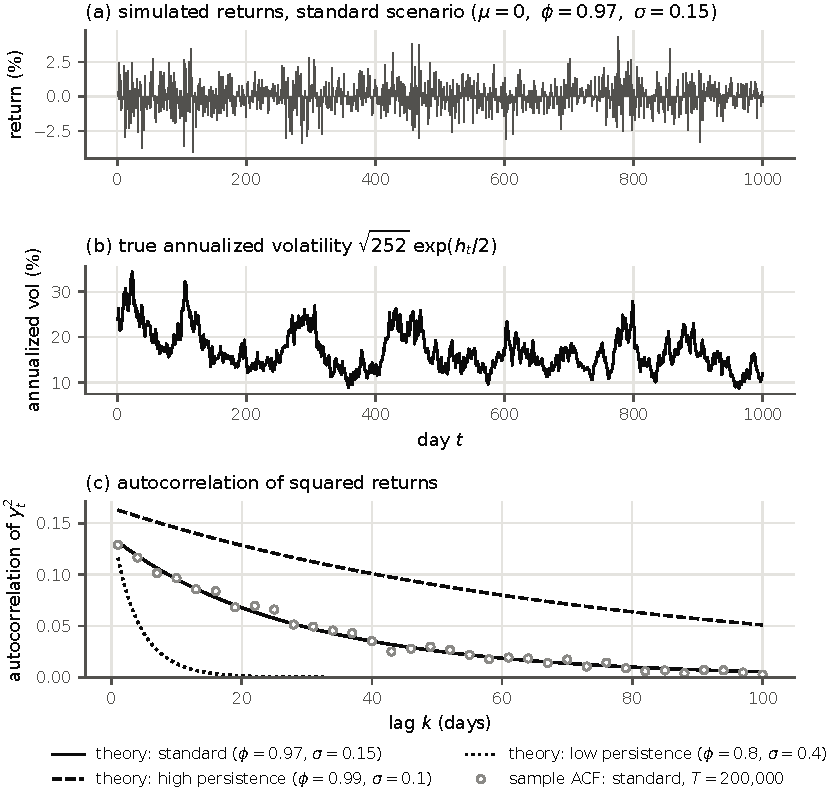
\includegraphics[width=\linewidth]{figures/fig1_sv_illustration.pdf}
  \caption{基本 SV モデルの例。(a) 標準シナリオ（$\mu = 0$、$\phi = 0.97$、$\sigma = 0.15$）から生成したリターン $y_t$（$T = 1{,}000$）。
    (b) その真の年率ボラティリティ $\sqrt{252}\exp(h_t/2)$。
    (c) 二乗リターンの自己相関。線は \cref{eq:sv-acf} による理論値（実線：標準、破線：高持続 $\phi = 0.99$、$\sigma = 0.10$、点線：低持続 $\phi = 0.8$、$\sigma = 0.4$）、
    白丸は標準シナリオの $T = 200{,}000$ の合成データから計算した標本自己相関（3 ラグごとに表示）。}
  \label{fig:sv-illustration}
\end{figure}

\cref{tab:sv-properties} は、合成データの 3 つのシナリオと、実データ（\cref{sec:empirical} の ETF 2 銘柄を NUTS で推定した事後平均）について、これらの量をまとめたものである。
合成データのシナリオは、いずれも $s \approx 0.6$〜$0.7$、尖度 4.4〜5.0 と裾の厚さは同程度だが、ショックの半減期が 3 日から 69 日まで大きく異なるように選んでいる。
実データの推定値は、$\phi$ が 0.86〜0.89 と合成データの標準シナリオより低く、$\sigma$ が 0.38〜0.46 と大きい。
その結果、半減期は 4〜6 日と短く、尖度は 6 を超える。
これは、推定に使った約 2 年の期間に 2025 年 4 月の急変動が含まれていることの影響が大きいと考えられる（\cref{sec:empirical} で改めて議論する）。

\begin{table}[tbp]
  \centering
  \caption{基本 SV モデルの定常的な性質。
    $s = \sqrt{\sigma^2/(1-\phi^2)}$ は対数ボラティリティの定常標準偏差、尖度は \cref{eq:sv-kurtosis} の $3e^{s^2}$、
    半減期は $\log 0.5 / \log\phi$、年率ボラの 95\% 範囲は定常分布 $h_t \sim \Normal(\mu, s^2)$ のもとでの $\sqrt{252}\exp(h_t/2)$ の 2.5\%・97.5\% 点。
    実データの行は \cref{sec:empirical} の NUTS による事後平均を代入した値。}
  \label{tab:sv-properties}
  \small
  \begin{tabular}{lrrrrrrr}
\toprule
 & $\mu$ & $\phi$ & $\sigma$ & $s$ & 尖度 & 半減期[日] & 年率ボラの95\%範囲[\%] \\
\midrule
合成：標準 & 0.00 & 0.970 & 0.150 & 0.617 & 4.39 & 22.8 & 8.7〜29.1 \\
合成：高持続 & 0.00 & 0.990 & 0.100 & 0.709 & 4.96 & 69.0 & 7.9〜31.8 \\
合成：低持続 & 0.00 & 0.800 & 0.400 & 0.667 & 4.68 & 3.1 & 8.3〜30.5 \\
\addlinespace
実データ：1321 & 0.61 & 0.889 & 0.384 & 0.840 & 6.07 & 5.9 & 9.5〜49.0 \\
実データ：1306 & 0.07 & 0.855 & 0.455 & 0.877 & 6.48 & 4.4 & 7.0〜38.9 \\
\bottomrule
\end{tabular}

\end{table}

\subsection{拡張 1：レバレッジ効果}\label{sec:model-leverage}

株式市場では、株価が下落した後にボラティリティが上昇しやすいという非対称性がよく知られており、\textbf{レバレッジ効果}と呼ばれる。
名前の由来は、株価が下がると企業の負債・自己資本比率（財務レバレッジ）が上がり、株式のリスクが高まるという説明である \parencite{christie1982}。
ほかにも、ボラティリティの上昇が予想されると投資家がより高いリスクプレミアムを求めて株価が下がる、という逆向きの因果による説明もある。
いずれの説明が正しいにせよ、下落局面でボラティリティが高まることは、VaR や ES のように損失側の裾を問題にする指標に直接影響するので、実務上重要な性質である。

SV モデルでは、レバレッジ効果を観測のショック $\varepsilon_t$ と状態のショック $\eta_t$ の相関として表す。本稿では
\begin{equation}
  y_t = \exp(h_t/2)\,\varepsilon_t, \qquad
  h_{t+1} = \mu + \phi\,(h_t - \mu) + \sigma\,\eta_t, \qquad
  \begin{pmatrix} \varepsilon_t \\ \eta_t \end{pmatrix} \sim \Normal\!\left( \begin{pmatrix} 0 \\ 0 \end{pmatrix}, \begin{pmatrix} 1 & \rho \\ \rho & 1 \end{pmatrix} \right)
  \label{eq:sv-leverage}
\end{equation}
とし、$\rho \in (-1, 1)$ を新たなパラメータとする（$t = T$ の $\varepsilon_T$ に対応する $\eta_T$ はモデルに現れない）。
$\rho < 0$ であれば、今日のリターンが負（$\varepsilon_t < 0$）のときに明日の対数ボラティリティへのショック $\eta_t$ が正になりやすく、レバレッジ効果が表される。

ここで重要なのは\textbf{時点の取り方}である。
\cref{eq:sv-leverage} では、今日の観測ショック $\varepsilon_t$ が、\textbf{明日}の対数ボラティリティ $h_{t+1}$ を動かすショック $\eta_t$ と相関する
\parencite{harvey1996,omori2007}。
これに対して、今日の $\varepsilon_t$ と今日の $h_t$ を動かすショック $\eta_{t-1}$ を相関させる定式化もある \parencite{jacquier2004}。
\textcite{yu2005} は二つの定式化を比較し、前者では $y_t$ がマルチンゲール差分（過去の情報のもとで条件付き平均が 0）になり、$\rho$ がレバレッジ効果の大きさとして素直に解釈できるのに対し、
後者ではそうならないことを示して、前者を支持している。本稿も前者を採用する。

実装と後の議論のために、\cref{eq:sv-leverage} を二通りの条件付き分布で書き直しておく。
二変量正規分布の条件付き分布の公式から、$\eta_t$ を与えたときの $\varepsilon_t$ は $\Normal(\rho\,\eta_t,\ 1-\rho^2)$ に、
$\varepsilon_t$ を与えたときの $\eta_t$ は $\Normal(\rho\,\varepsilon_t,\ 1-\rho^2)$ に従う。
\begin{enumerate}[label=(\alph*)]
  \item \textbf{観測を状態で条件付ける形}：$h_t$ と $h_{t+1}$ が分かれば $\eta_t = \{h_{t+1} - \mu - \phi(h_t - \mu)\}/\sigma$ が決まるので、
    \begin{equation}
      y_t \mid h_t, h_{t+1} \sim \Normal\!\left(\rho\, e^{h_t/2}\, \eta_t,\ (1-\rho^2)\, e^{h_t}\right) \quad (t < T), \qquad
      y_T \mid h_T \sim \Normal(0,\ e^{h_T}).
      \label{eq:sv-leverage-obs}
    \end{equation}
    $h_{1:T}$ の周辺分布は基本 SV と同じ AR(1) 過程であり（$\eta_t$ の周辺分布は $\Normal(0, 1)$ のまま）、
    同時分布は $p(h_{1:T} \mid \theta) \prod_{t} p(y_t \mid h_t, h_{t+1}, \theta)$ と分解できる。
    本稿の実装（尤度の計算）はこの形を使う。
  \item \textbf{状態を観測で条件付ける形}：今日のリターン $y_t$ が分かれば $\varepsilon_t = y_t\, e^{-h_t/2}$ が決まるので、
    \begin{equation}
      h_{t+1} \mid h_t, y_t \sim \Normal\!\left(\mu + \phi\,(h_t - \mu) + \rho\,\sigma\, y_t\, e^{-h_t/2},\ \ \sigma^2 (1-\rho^2)\right).
      \label{eq:sv-leverage-state}
    \end{equation}
    明日の対数ボラティリティは、基本 SV の AR(1) の予測に、今日の標準化リターンに比例する項 $\rho\sigma\, y_t e^{-h_t/2}$ を足したものになる。
    $\rho < 0$ なら、大きな下落の翌日には対数ボラティリティが押し上げられる。
    同時に、予測の不確実性は $\sigma^2$ から $\sigma^2(1-\rho^2)$ に小さくなる（今日のリターンが明日のボラティリティの情報を含むため）。
    この形は、1 期先の予測（\cref{sec:model-predictive}）と、\cref{sec:family} で条件付き構造化変分族をレバレッジ SV に拡張するときに使う。
\end{enumerate}

\subsection{拡張 2：$t$ 分布の誤差}\label{sec:model-t}

基本 SV モデルは、ボラティリティの変動によって周辺分布の裾を厚くするが、各日の条件付き分布は正規分布のままである。
しかし実際のリターンには、その日のボラティリティの水準から見ても極端に大きな変動（例えば突然のニュースによる急落）が含まれることがある。
これを表すために、観測ショック $\varepsilon_t$ を、分散が 1 になるように基準化した自由度 $\nu$ の $t$ 分布に置き換える \parencite{chib2002,jacquier2004}。
\begin{equation}
  y_t = \exp(h_t/2)\,\varepsilon_t, \qquad \varepsilon_t = \sqrt{\frac{\nu-2}{\nu}}\; u_t, \qquad u_t \sim t_\nu, \qquad \nu > 2.
  \label{eq:sv-t}
\end{equation}
自由度 $\nu$ の $t$ 分布の分散は $\nu/(\nu-2)$ なので、係数 $\sqrt{(\nu-2)/\nu}$ を掛けると $\varepsilon_t$ の分散は 1 になる。
この基準化により、$h_t$ は基本 SV と同じく「日次分散の対数」という意味を保ち、$\nu$ は分散を変えずに裾の厚さだけを表すパラメータになる。
基準化には分散が有限であること、すなわち $\nu > 2$ が必要である。
状態方程式 \cref{eq:sv-state,eq:sv-init} は基本 SV と同じである。

観測の対数尤度は
\[
  \log p(y_t \mid h_t, \nu) = \log \Gamma\!\left(\tfrac{\nu+1}{2}\right) - \log \Gamma\!\left(\tfrac{\nu}{2}\right) - \frac{1}{2}\log\{\pi(\nu-2)\}
    - \frac{h_t}{2} - \frac{\nu+1}{2} \log\!\left(1 + \frac{y_t^2\, e^{-h_t}}{\nu - 2}\right)
\]
である。
$t$ 分布は、正規分布の分散を逆ガンマ分布に従って確率的に変えた混合分布として
$\varepsilon_t = \sqrt{(\nu-2)\lambda_t/\nu}\; z_t$、$z_t \sim \Normal(0,1)$、$\lambda_t \sim \mathrm{InvGamma}(\nu/2,\ \nu/2)$
とも書ける。MCMC ではこの表現で $\lambda_t$ を潜在変数として加えることが多いが、本稿では $\lambda_t$ を積分消去した上の密度をそのまま使う
（変分推論では、潜在変数を増やさずに直接扱える方が素直だからである）。

$t$ 誤差の SV モデルの尖度は、$\nu > 4$ のとき
\[
  \kappa = 3\,\frac{\nu-2}{\nu-4}\; e^{s^2}
\]
であり、ボラティリティの変動による部分 $e^{s^2}$ と、各日の条件付き分布の裾による部分 $(\nu-2)/(\nu-4)$ の積になる。
二つの拡張の役割を整理すると、基本 SV がボラティリティの「ゆっくりした」変動を、$t$ 誤差がボラティリティの水準では説明できない「単発の」大きな変動を担当する、という分担になる。
どちらがデータの裾の厚さをどれだけ説明するかは、推定してみて初めて分かる（実データでは $\nu$ の事後平均が 20〜25 と大きく、裾の厚さはほぼボラティリティの変動で説明された。\cref{sec:empirical}）。

なお本稿では、レバレッジ効果と $t$ 誤差を同時に持つモデルは扱わない。
両者を組み合わせるには、$\varepsilon_t$ と $\eta_t$ の同時分布を（二変量正規分布ではなく）別の形で定める必要があり、モデルと推定の両面で議論が増えるためである。

\subsection{事前分布}\label{sec:model-prior}

ベイズ推定では、パラメータ $\theta$ に事前分布を置く。本稿で使う事前分布を \cref{tab:priors} にまとめる。

\begin{table}[tbp]
  \centering
  \caption{事前分布と、その平均・95\% 区間（2.5\%・97.5\% 点）。$\sigma$ の事前分布は半正規分布を標準とし、逆ガンマ分布（$\sigma^2$ に対する）は感度分析（\cref{app:settings}）でのみ使う。}
  \label{tab:priors}
  \small
  \begin{tabular}{llrl}
\toprule
パラメータ & 事前分布 & 事前平均 & 95\% 区間 \\
\midrule
$\mu$ & $\Normal(0,\ 10^2)$ & 0.0 & [-19.6,\ 19.6] \\
$\phi$ & $(\phi+1)/2 \sim \mathrm{Beta}(20,\ 1.5)$ & 0.860 & [0.588,\ 0.989] \\
$\sigma$ & $\mathrm{HalfNormal}(1)$（標準） & 0.798 & [0.031,\ 2.241] \\
$\sigma$ & $\sigma^2 \sim \mathrm{InvGamma}(2.5,\ 0.025)$（感度分析） & 0.119 & [0.062,\ 0.245] \\
$\rho$ & $\mathrm{Uniform}(-1,\ 1)$ & 0.000 & [-0.95,\ 0.95] \\
$\nu$ & $\nu-2 \sim \mathrm{Gamma}(2,\ 0.1)$ & 22.0 & [4.4,\ 57.7] \\
\bottomrule
\end{tabular}

\end{table}

\begin{itemize}
  \item $\mu \sim \Normal(0, 10^2)$：\% 単位では $\mu$ は $-1$〜$2$ 程度なので、標準偏差 10 は実質的に情報を持たない（弱情報の）事前分布である。
  \item $(\phi + 1)/2 \sim \mathrm{Beta}(20, 1.5)$：\textcite{kim1998} 以来、SV モデルで標準的に使われている事前分布である。
    $\phi$ を $(-1, 1)$ に収めつつ、日次データで典型的な高い持続性に事前の重みを置く（事前平均 0.86、95\% 区間 $[0.59, 0.99]$）。
    実データの推定値（0.86〜0.89）はこの区間の中央付近にある。一方、高持続シナリオの真値 0.99 は区間の上端にあたり、事前分布が $\phi$ をわずかに下に引く方向に働く。
  \item $\sigma \sim \mathrm{HalfNormal}(1)$（半正規分布）：$\sigma^2$ に $\chi^2_1$ 分布（形状 1/2 のガンマ分布）を置くことと同じであり、
    \textcite{kastner2014} でも使われている。
    \textcite{kim1998} は $\sigma^2$ に逆ガンマ分布 $\mathrm{InvGamma}(2.5,\ 0.025)$ を置いたが、逆ガンマ分布は $\sigma = 0$ の近くで密度が 0 になり、$\sigma$ を 0 から遠ざける方向に働く。
    また \cref{tab:priors} のとおり、この逆ガンマ分布は $\sigma$ の 95\% 区間が $[0.06, 0.25]$ と狭く、実データの推定値（0.38〜0.46）はその外側にある。
    半正規分布は $\sigma = 0$ の近くでも正の密度を持ち、かつ 0.03〜2.2 という広い範囲を覆うので、本稿ではこちらを標準とする。
    逆ガンマ分布は合成データでの感度分析にのみ使い、提案手法の推定結果が事前分布の選び方でほとんど変わらないことを確認している（\cref{app:settings}）。
  \item $\rho \sim \mathrm{Uniform}(-1, 1)$：レバレッジの向きと大きさについて事前に特定の値を仮定しない。
  \item $\nu - 2 \sim \mathrm{Gamma}(2,\ 0.1)$（形状 2、レート 0.1）：自由度の事前分布として広く使われる $\mathrm{Gamma}(2, 0.1)$ \parencite{juarez2010} を、
    基準化に必要な $\nu > 2$ を満たすように 2 だけずらしたものである。事前平均は 22、95\% 区間は $[4.4, 57.7]$ で、裾の厚い分布（$\nu \approx 5$）から正規分布に近い分布（$\nu > 30$）までを覆う。
\end{itemize}

事前分布は、データが十分にあれば推定結果にほとんど影響しないが、本稿の実データのように系列が短い（約 500 日）場合には無視できないことがある。
とくに $\nu$ は裾の観測が少ないと事後分布が事前分布からあまり動かず、実データでの $\nu$ の推定値はこの点を割り引いて読む必要がある（\cref{sec:empirical}）。

\subsection{尤度が解析的に書けない理由と事後分布}\label{sec:model-likelihood}

パラメータ $\theta$ の尤度は、\cref{eq:sv-joint} を潜在変数 $h_{1:T}$ について積分した
\begin{equation}
  p(y_{1:T} \mid \theta) = \int p(y_{1:T} \mid h_{1:T})\, p(h_{1:T} \mid \theta)\, dh_{1:T}
  \label{eq:sv-marginal}
\end{equation}
である。これは $T$ 次元の積分であり、閉じた形では計算できない。

もし観測方程式が $h_t$ について線形で、誤差が正規分布であれば、\cref{eq:sv-marginal} はカルマンフィルタによって $O(T)$ の計算量で厳密に計算できる。
SV モデルの観測方程式は、$y_t$ の分散が $e^{h_t}$ という形で $h_t$ に非線形に依存しており、この条件を満たさない。
両辺を二乗して対数をとると
\[
  \log y_t^2 = h_t + \log \varepsilon_t^2
\]
と $h_t$ について線形になるが、誤差 $\log \varepsilon_t^2$ は $\log \chi^2_1$ 分布という左に長い裾を持つ非正規分布に従う（平均 $\approx -1.27$、分散 $\pi^2/2 \approx 4.93$）。
これを正規分布で置き換えてカルマンフィルタを使うのが疑似最尤法（QML）\parencite{harvey1994} であり、
$\log \chi^2_1$ 分布を正規分布の混合で精度よく近似して MCMC に組み込んだのが \textcite{kim1998} である。

この変形は、SV モデルの推定が難しいもう一つの理由も教えてくれる。
1 日分の観測 $\log y_t^2$ に含まれる $h_t$ の情報は、分散 4.93 という大きなノイズに埋もれている。
一方、$h_t$ 自体の変動の大きさは定常分散 $s^2$ でおよそ 0.4〜0.8 にすぎない（\cref{tab:sv-properties}）。
つまり 1 日の観測だけでは $h_t$ はほとんど決まらず、\textbf{$h_t$ の推定は、前後の多くの日の観測を AR(1) の構造を通じて平滑化することで初めて可能になる}。
これは、$h_t$ の事後分布で隣り合う日どうしが強く相関することを意味しており、\cref{sec:family} で平均場近似が失敗する理由そのものである。

ベイズ推定では、積分 \cref{eq:sv-marginal} を直接計算する代わりに、潜在変数 $h_{1:T}$ もパラメータと一緒に未知数として扱い、同時事後分布
\begin{equation}
  p(\theta, h_{1:T} \mid y_{1:T}) \;\propto\; p(\theta)\; p(h_{1:T} \mid \theta)\; p(y_{1:T} \mid h_{1:T}, \theta)
  \label{eq:sv-posterior}
\end{equation}
を考える。右辺は \cref{eq:sv-loglik} などの初等的な関数の積なので、正規化定数を除けばいつでも計算できる。
求めたいのは $\theta$ と $h_{1:T}$ の事後分布（の要約）であり、その次元は $T + k$（$k$ は大域パラメータの数で、基本 SV で 3、拡張モデルで 4）である。
本稿の実データ（$T = 485$）でも約 500 次元、10 年分の日次データなら約 2,500 次元になる。
\cref{sec:inference} で述べる MCMC と変分推論は、いずれもこの高次元の事後分布 \cref{eq:sv-posterior} を扱う方法である。

なお、観測の対数尤度 \cref{eq:sv-loglik} は $h_t$ について凹関数である（2 階微分が $-y_t^2 e^{-h_t}/2 \leq 0$）。
$t$ 誤差の場合も、$a_t = y_t^2/(\nu-2)$、$u_t = a_t e^{-h_t}$ とおくと 2 階微分は $-\frac{\nu+1}{2}\,\frac{u_t}{(1+u_t)^2} \leq 0$ で、やはり凹である。
AR(1) の事前分布も $h_{1:T}$ について凹（対数が二次形式）なので、$\theta$ を固定したときの $h_{1:T}$ の事後分布は単峰で、正規分布による近似がよく効く。
二つのモデルの曲率を比べると、正規誤差では大きなリターン $y_t$ ほど曲率 $y_t^2 e^{-h_t}/2$ が際限なく大きくなり、1 日の極端なリターンが $h_t$ を強く引き寄せる。
$t$ 誤差では曲率が $(\nu+1)/8$ 以下に抑えられ、極端なリターンの影響が自動的に割り引かれる（頑健になる）。
また、リターンがちょうど 0 の日（売買が少ない銘柄などで生じる）は、正規誤差の対数尤度が $-h_t/2$ だけになり単独では $h_t \to -\infty$ を好むが、AR(1) の事前分布が $h_t$ を前後の日の水準に引き留めるので、推定上の問題にはならない。

\subsection{事後分布の構造：三重対角の精度行列}\label{sec:model-structure}

\cref{sec:family} で変分族を設計するために、事後分布 \cref{eq:sv-posterior} の構造をもう少し詳しく見ておく。
鍵になるのは、正規分布の\textbf{精度行列}（共分散行列の逆行列）である。
多変量正規分布では、精度行列の $(i, j)$ 成分が 0 であることと、「他のすべての変数を与えたとき、$i$ 番目と $j$ 番目の変数が条件付き独立であること」が同値になる。
したがって、変数間の条件付き独立性が多ければ精度行列は疎（0 の多い行列）になる。

\paragraph{AR(1) の事前分布の精度行列}
\cref{eq:sv-state,eq:sv-init} の定常 AR(1) 過程では、$h_t$ は直前の $h_{t-1}$ と直後の $h_{t+1}$ を与えれば、それ以外の日と条件付き独立である。
実際、$p(h_{1:T} \mid \theta)$ の対数は $h_{1:T}$ の二次形式であり、$h - \mu\mathbf{1}$ についての精度行列は
\begin{equation}
  Q_{\mathrm{AR}}(\phi, \sigma) = \frac{1}{\sigma^2}
  \begin{pmatrix}
    1      & -\phi    &        &        &        \\
    -\phi  & 1+\phi^2 & -\phi  &        &        \\
           & \ddots   & \ddots & \ddots &        \\
           &          & -\phi  & 1+\phi^2 & -\phi \\
           &          &        & -\phi  & 1
  \end{pmatrix}
  \label{eq:ar1-precision}
\end{equation}
という\textbf{三重対角行列}になる（空白の成分は 0）。
左上の成分は、定常分布の精度 $(1-\phi^2)/\sigma^2$ と、$h_2$ の式から来る $\phi^2/\sigma^2$ の和として $1/\sigma^2$ になる。
共分散行列（$\mathrm{Cov}(h_s, h_t) = s^2 \phi^{|s-t|}$）は密な行列であるのに、精度行列はこのように疎である。

\paragraph{$\theta$ を固定したときの $h$ の事後分布}
次に、$\theta$ を固定して $h_{1:T}$ の事後分布 $p(h_{1:T} \mid y_{1:T}, \theta)$ を考える。
その対数は、AR(1) の事前分布の対数（三重対角の二次形式）と、各日の観測の対数尤度の和 $\sum_t \log p(y_t \mid h_t)$ からなる。
後者は $h_t$ ごとに分かれた和なので、$h_{1:T}$ についてのヘッセ行列（2 階微分の行列）は\textbf{対角行列}である。
したがって、事後分布の最頻値 $\hat h$ のまわりで二次近似（ラプラス近似）をすると、近似した正規分布の精度行列は
\begin{equation}
  Q_{\mathrm{AR}}(\phi, \sigma) + \diag\!\left( \frac{y_1^2}{2}\,e^{-\hat h_1}, \dots, \frac{y_T^2}{2}\,e^{-\hat h_T} \right)
  \label{eq:laplace-precision}
\end{equation}
となり、やはり三重対角である。
つまり、$\theta$ を与えたときの $h$ の事後分布は、「AR(1) の事前分布」に「各日ごとの正規分布の形をした情報」を掛け合わせたもので、よく近似できる。
\cref{sec:family} の条件付き構造化変分族は、まさにこの形（各日の情報の位置と精度を変分パラメータとして最適化する）を変分族として採用したものである。

$t$ 誤差のモデルでも観測の対数尤度は $h_t$ ごとに分かれるので、構造は同じである。
レバレッジ SV では、\cref{eq:sv-leverage-obs} のとおり $y_t$ の尤度が $h_t$ と $h_{t+1}$ の両方に依存するが、依存するのは隣り合う日の組だけなので、
ヘッセ行列への寄与は $(t, t)$、$(t, t+1)$、$(t+1, t+1)$ 成分に限られ、\textbf{三重対角の帯構造は保たれる}（ただし、各日の寄与が凹であるとは限らない）。

三重対角の精度行列を持つ正規分布は、コレスキー分解・前進代入・後退代入をすべて $O(T)$ の計算量で行える。
したがって、密度の計算・サンプリング・エントロピーの計算をすべて $O(T)$ で行える。
これは、MCMC で状態を一括してサンプリングするために \textcite{chan2009} が使った性質であり、本稿では変分族の側で利用する（\cref{sec:family}）。

\paragraph{パラメータと状態の事後的な依存}
同時事後分布 \cref{eq:sv-posterior} では、$\theta$ と $h_{1:T}$ も互いに強く依存する。
\begin{itemize}
  \item \textbf{$\sigma$ と $h$ の滑らかさ}：\cref{eq:laplace-precision} のとおり、$h$ の事後分布の精度行列の大部分は $1/\sigma^2$ に比例する。
    $\sigma$ が小さいと考えるなら $h$ の経路は滑らかでなければならず、$\sigma$ が大きいと考えるなら $h$ は日々大きく動いてよい。
    $\sigma$ の不確実性を正しく表すには、$h$ の経路の滑らかさが $\sigma$ に連動して変わる必要がある。
  \item \textbf{$\mu$ と $h$ の水準}：$\mu$ を大きく見積もるなら、$h$ 全体も上に動く。
  \item \textbf{$\mu$ と $\phi$}：$\mu$ は $h_t$ が戻っていく先の水準なので、$h_t$ の平均回帰が速い（$\phi$ が小さい）ほどよく決まり、$\phi$ が 1 に近いほど決まりにくい。
    AR(1) 過程の標本平均の分散がおよそ $\sigma^2 / \{(1-\phi)^2 T\}$ であることからも分かるように、$\phi$ が 1 に近づくと $\mu$ の事後分布の幅は急速に広がる。
    例えば実データの 1321 の推定値（$\phi \approx 0.89$、$\sigma \approx 0.38$、$T = 485$）では、この式から $\mu$ の不確実性は標準偏差で約 0.16 と見積もられ、NUTS による事後標準偏差 0.21 と同程度の大きさになる。
    この結果、$(\mu, \phi)$ の同時事後分布は、$\phi$ が大きいところほど $\mu$ の方向に広がる「バナナ型」の形になり、正規分布ではうまく表せない。
\end{itemize}
これらの依存は、$\theta$ と $h$ を独立とみなす変分族では表現できない。
\cref{sec:family,sec:synthetic} で見るように、とくに $\sigma$ と $h$ の依存を無視すると、$\sigma$ の不確実性が大きく過小評価される。

\subsection{パラメータ化：中心化と非中心化}\label{sec:model-param}

同じ SV モデルでも、潜在変数を何に取るか（\textbf{パラメータ化}）によって、推定のしやすさが大きく変わる。
ここまでの定式化のように $h_{1:T}$ そのものを潜在変数とするものを\textbf{中心化パラメータ化}と呼ぶ。
これに対して、標準化した
\[
  x_t = \frac{h_t - \mu}{\sigma}, \qquad
  x_1 \sim \Normal\!\left(0, \frac{1}{1-\phi^2}\right), \quad x_{t+1} = \phi\, x_t + \eta_t, \qquad h_t = \mu + \sigma\, x_t
\]
を潜在変数とするものを\textbf{非中心化パラメータ化}と呼ぶ。
二つは同じ確率モデルの異なる表現であり、事後分布から計算される $h_t$ や $\theta$ の分布は（推定が正確であれば）一致する。
違うのは、推定アルゴリズムから見た事後分布の「形」である。
中心化では、事前分布の段階で $h$ が $\mu$・$\sigma$ に依存する（$\mu$ と $\sigma$ が $h$ の水準と滑らかさを決める）。
非中心化では、事前分布の段階では $x$ と $(\mu, \sigma)$ が独立になり、依存は観測の尤度を通じてだけ生じる。

一般に、データが潜在変数についての情報を多く含むときは中心化が、少ないときは非中心化が、MCMC の効率の点で有利になることが知られている \parencite{papaspiliopoulos2007}。
SV モデルでは、どちらが有利かがパラメータの値やデータによって変わり、
\textcite{kastner2014} の ASIS は、二つのパラメータ化を交互に使うことで両方の長所を取り入れる方法である。

本稿の予備実験では、持続性の高いシナリオ（$\phi = 0.99$、$T = 1{,}000$）で、非中心化の NUTS は $\mu$ がほとんど混合せず（ESS は約 10、$\hat R = 1.66$）、
中心化の NUTS では $\mu$ の ESS が約 3,000 と良好だった（一方で、$\sigma$ の ESS は約 80 と低めだった）。
そこで本稿では、「正解」として使う NUTS には中心化パラメータ化を採用し、混合の悪さを補うために反復を長くとる（\cref{sec:synthetic}）。

変分推論でも、パラメータ化の選択は結果に影響しうる。
平均場近似や、$\theta$ と $h$ を独立とする構造化近似では、どちらのパラメータ化で変分族を当てるかによって近似の結果が変わる（\cref{app:settings}）。
一方、\cref{sec:family} の条件付き構造化変分族は、$\theta$ を固定すると $h = \mu + \sigma x$ がアフィン変換であることから、\textbf{どちらのパラメータ化を使っても同じ分布族になる}。
パラメータ化という調整項目を一つ減らせることは、システムとして運用するうえでの利点でもある。

\subsection{1 期先の予測分布と VaR}\label{sec:model-predictive}

最後に、\cref{sec:empirical} の VaR のバックテストで使う 1 期先の予測分布を定義する。
時点 $T$ までのデータ $y_{1:T}$ をもとにした翌日のリターン $y_{T+1}$ の予測分布は、
\begin{equation}
  p(y_{T+1} \mid y_{1:T}) = \int p(y_{T+1} \mid h_{T+1}, \theta)\; p(h_{T+1} \mid h_T, y_T, \theta)\; p(\theta, h_T \mid y_{1:T})\; d\theta\, dh_T\, dh_{T+1}
  \label{eq:predictive}
\end{equation}
である。ここで $p(\theta, h_T \mid y_{1:T})$ は同時事後分布 \cref{eq:sv-posterior} の $(\theta, h_T)$ についての周辺分布であり、
最終時点 $h_T$ については、これは「時点 $T$ までの情報で見た今日の対数ボラティリティの分布」（フィルタリング分布）に一致する。
$p(h_{T+1} \mid h_T, y_T, \theta)$ は、基本 SV と $t$ 誤差のモデルでは状態方程式 \cref{eq:sv-state} そのもの（$y_T$ には依存しない）、
レバレッジ SV では \cref{eq:sv-leverage-state} である。
レバレッジ SV では、今日のリターン $y_T$ が負で大きいほど翌日のボラティリティの予測が上がり、VaR が保守的になる。

実際の計算では、MCMC のサンプル、または変分分布から生成したサンプル $(\theta^{(s)}, h_T^{(s)})$、$s = 1, \dots, S$ を使う。
各サンプルについて $h_{T+1}^{(s)}$ を状態方程式から 1 つ生成すると、予測分布は
\[
  p(y_{T+1} \mid y_{1:T}) \approx \frac{1}{S} \sum_{s=1}^{S} p\!\left(y_{T+1} \mid h_{T+1}^{(s)}, \theta^{(s)}\right)
\]
という $S$ 個の正規分布（$t$ 誤差のモデルでは $t$ 分布）の混合で近似できる。
この混合分布は、パラメータの不確実性と今日・明日のボラティリティの不確実性をすべて反映しているので、単一の正規分布より裾が厚い。
有意水準 $\alpha$（本稿では 5\% と 1\%）の VaR は、この混合分布の下側 $\alpha$ 分位点、すなわち
\[
  \frac{1}{S} \sum_{s=1}^{S} F\!\left(q \mid h_{T+1}^{(s)}, \theta^{(s)}\right) = \alpha
\]
を満たす $q$ として計算する（$F$ は各成分の累積分布関数。$q$ は 1 次元の方程式なので二分法などで確実に解ける）。
本稿では VaR をリターンの分位点（負の値）として表し、実現リターンが VaR を下回った日を「超過」と数える。
また、予測分布の良さを分位点だけでなく分布全体で評価するために、実現値 $y_{T+1}^{\mathrm{obs}}$ での対数予測密度（対数予測スコア）
\[
  \log p(y_{T+1}^{\mathrm{obs}} \mid y_{1:T}) \approx \log \frac{1}{S} \sum_{s=1}^{S} p\!\left(y_{T+1}^{\mathrm{obs}} \mid h_{T+1}^{(s)}, \theta^{(s)}\right)
\]
も計算する（大きいほど良い）。
混合分布の密度と累積分布関数を直接計算するので、$y_{T+1}$ をさらに乱数で生成して分位点を求めるより、モンテカルロ誤差が小さい。
推定方法（NUTS か変分推論か、どの変分族か）の違いは、すべてサンプル $(\theta^{(s)}, h_T^{(s)})$ の分布の違いとして予測分布に反映される。
とくに、変分推論が $\theta$ や $h_T$ の不確実性を過小評価すると、予測分布の裾が薄くなり、VaR の超過が増えることになる。

% 3 章：事後分布、NUTS、KL と ELBO、再パラメータ化勾配、ADVI
\section{ベイズ推定と変分推論の基礎}\label{sec:inference}

（執筆予定）

% 4 章：SV モデルのための変分族
% 記述は実装と一致させている：src/sv_vi/advi.py（3 つの自前の族、conditional_factor）、banded.py（三重対角の O(T) 演算）、
% initialization.py（初期値）、guides.py（NumPyro 側の族）。
% 図 fig_sigma_roughness・表 tab_families は experiments/f4_family_illustration.py が生成。
\section{SV モデルのための変分族}\label{sec:family}

本章は本稿の中心であり、SV モデルの事後分布を近似する変分族を定義し、その性質を比較する。
\cref{sec:fam-requirements}で、第 2・3 章の議論から変分族に求められる要件を整理する。
\cref{sec:fam-meanfield,sec:fam-dense}で、汎用的な族（平均場、低ランク、フルランク）がなぜ SV モデルに向かないかを述べ、
\cref{sec:fam-structured}で、事後分布の三重対角構造を取り入れた構造化族と、その限界を説明する。
\cref{sec:fam-conditional}で、本稿が提案として扱う条件付き構造化族を定義し、
\cref{sec:fam-leverage,sec:fam-t}でそれを二つの拡張モデルに適用する。
\cref{sec:fam-summary}で各族を比較し、\cref{sec:fam-init}で初期値の設定を述べる。

本章では、第 3 章の ADVI に従い、大域パラメータを無制約空間の変数 $u \in \mathbb{R}^k$（$\theta = \theta(u)$）で表し、
推定する未知数を $z = (u, h_{1:T})$ とする（非中心化パラメータ化では $h$ の代わりに $x$）。
$k$ は大域パラメータの数で、基本 SV では 3、拡張モデルでは 4 である。

\subsection{変分族に求められる要件}\label{sec:fam-requirements}

第 2・3 章の議論から、SV モデルの変分族には次の四つが求められる。

\begin{enumerate}[label=(R\arabic*)]
  \item \textbf{$h_t$ の時間方向の相関を表せること}。
    $\theta$ を固定しても、隣り合う日の $h_t$ の事後相関は 0.9 程度に達する（\cref{tab:meanfield-gap}）。
    これを表せない族は、不確実性を過小評価するだけでなく、ELBO を通じてパラメータの推定そのものを偏らせる（\cref{sec:inf-vi}）。
  \item \textbf{$\theta$ と $h$ の事後的な依存を表せること}。
    とくに、$\sigma$ が $h$ の経路の滑らかさを決め、$\mu$ が $h$ の水準を決めるという依存（\cref{sec:model-structure}）である。
    これを表せないと、$\sigma$ の推定が偏り、その不確実性が過小評価される（\cref{sec:fam-structured}）。
  \item \textbf{計算量が $O(T)$ であること}。
    系列長 $T$ は数百〜数千であり、多数の銘柄を毎日推定することを考えると、1 ステップの計算量が $T$ の 2 乗以上で増える族は使いにくい。
    変分パラメータの数も $O(T)$ に抑えたい。数が多すぎると、雑音のある勾配での最適化が難しくなる。
  \item \textbf{パラメータ化の選び方に結果が左右されにくいこと}。
    中心化と非中心化のどちらを使うべきかを、銘柄やデータ期間ごとに判断しなくて済むことが、運用上は望ましい（\cref{sec:model-param}）。
\end{enumerate}

\cref{sec:model-structure}で見たように、(R1) と (R3) を同時に満たす鍵は、$h$ の事後分布の精度行列が三重対角であることにある。
(R2) を満たすには、$h$ の変分分布が $\theta$ に依存する形にしなければならない。
以下では、この観点から族を順に見ていく。

\subsection{平均場近似}\label{sec:fam-meanfield}

最も単純な族は、すべての変数を互いに独立な正規分布とする平均場近似である。
\[
  q(z) = \prod_{i=1}^{k} \Normal(u_i \mid m_i, s_i^2) \prod_{t=1}^{T} \Normal(h_t \mid m_{k+t}, s_{k+t}^2).
\]
変分パラメータは各変数の平均と標準偏差（正値を保つため対数で持つ）で、数は $2(k + T)$ である。
サンプリングは $z_i = m_i + s_i \epsilon_i$、エントロピーは $\sum_i \log s_i + \frac{k+T}{2}(1 + \log 2\pi)$ であり、計算量は $O(T)$ と最も軽い。
NumPyro の \code{AutoNormal} はこの族である。

しかし平均場近似は (R1) も (R2) も満たさない。
\cref{sec:inf-vi}で示したとおり、$h_t$ の時間方向の相関を表せないことから、ELBO は平均場近似が正確になる小さい $\phi$ を好み、
持続性の高いシナリオで $\phi$ を 0.05 程度にまで崩してしまう（真値 0.99）。
$\phi$ が崩れると、モデルは $h_t$ を日々ほぼ独立に動くものと解釈するので、$\sigma$ は 0.70 と真値（0.10）の 7 倍になり、
$h_t$ の事後標準偏差は NUTS の約 2 倍になる（\cref{sec:synthetic}）。
つまり平均場近似では、$h_t$ の不確実性はむしろ過大になり、「不確実性を過小評価する」という一般論とは逆の現れ方をする。
いずれにしても推定は使い物にならない。

\subsection{低ランク近似とフルランク近似}\label{sec:fam-dense}

平均場の対極にあるのが、すべての変数間の相関を許すフルランクの正規分布である。
\[
  q(z) = \Normal(z \mid m,\ L L^\top), \qquad L \text{ は対角が正の下三角行列}.
\]
次元を $d = k + T$ とすると、変分パラメータの数は $d + d(d+1)/2$ であり、$T = 1{,}000$ では約 50 万になる。
サンプリング $z = m + L\epsilon$ は $O(d^2)$、$\log q(z)$ の計算は三角行列の方程式を解くので $O(d^2)$ の計算量とメモリを要する。
族としては真の事後分布の正規近似を含むので、最適化が完全にできれば平均場よりはるかに良い近似が得られるはずである。
しかし実際には、50 万個のパラメータを、1 ステップ 4 サンプルの雑音のある勾配で最適化するのは難しい。
本稿の実験（NumPyro の \code{AutoMultivariateNormal}、20,000 ステップ）では、230 秒かけても $\phi = 0.24$ にとどまり、ELBO は比較したすべての族の中で最も低かった（\cref{sec:synthetic}）。

その中間として、共分散行列を「低ランク行列 + 対角行列」で表す低ランク近似がある。
\[
  q(z) = \Normal(z \mid m,\ W W^\top + D), \qquad W \in \mathbb{R}^{d \times r},\ D \text{ は対角}.
\]
本稿では NumPyro の \code{AutoLowRankMultivariateNormal} をランク $r = 10$ で使う。パラメータ数は $d(r+2)$、計算量は $O(d r)$（逆行列はウッドベリーの公式で計算）である。
低ランク近似は、少数の「共通因子」で多くの変数が一斉に動くような相関（例えば、全体の水準が上下する）を表すのは得意である。
しかし SV モデルの $h_t$ の相関は、隣り合う日どうしが強く、日が離れるにつれてなめらかに弱まる、という\textbf{局所的な}相関である。
AR(1) 過程の共分散行列の固有値は、周波数ごとのスペクトル密度 $\sigma^2/(1 - 2\phi\cos\omega + \phi^2)$ に対応してゆっくりと減衰するので、
少数の成分では局所的な相関を表しきれない。
実際、ランク 10 の低ランク近似は、平均場とほぼ同じ $\phi = 0.05$ に崩れた（\cref{sec:synthetic}）。

この二つの例は、\textbf{パラメータを増やすことと、事後分布の構造に合った族を選ぶことは別である}ことを示している。

\subsection{構造化近似：三重対角の精度行列}\label{sec:fam-structured}

\cref{sec:model-structure}で見たように、$\theta$ を固定したときの $h$ の事後分布は、三重対角の精度行列を持つ正規分布でよく近似できる。
そこで、$h$ の変分分布として、三重対角の精度行列を持つ正規分布を使う。
大域パラメータは次元が小さい（$k = 3$〜$4$）ので、フルランクの正規分布で表す。
\begin{equation}
  q(u, h) = \Normal(u \mid m_u,\ C C^\top)\; \Normal\!\left(h \mid m_h,\ (L L^\top)^{-1}\right).
  \label{eq:fam-structured}
\end{equation}
$C$ は $k \times k$ の下三角行列、$L$ は\textbf{下二重対角行列}（対角 $d_1, \dots, d_T > 0$ と、そのすぐ下の副対角 $s_1, \dots, s_{T-1}$ だけが 0 でない行列）である。
このとき精度行列 $L L^\top$ は三重対角になり、逆に三重対角の正定値行列は必ずこの形に分解できる（コレスキー分解）。
変分パラメータは $m_u$、$C$、$m_h$、$\log d_t$、$s_t$ で、数は $k + k(k+1)/2 + 3T - 1$ である。
この族は、精度行列のコレスキー因子に疎な構造を課した \textcite{tan2018} の変分近似の一例であり、\textcite{archer2015} の構造化近似とも同じ考え方に立つ。
本稿では、自前実装（\code{advi.py} の \code{structured}）と NumPyro のガイド（\code{guides.py}）の両方で実装し、同じ結果が得られることを確認した（\cref{sec:synthetic}）。

\paragraph{$O(T)$ の計算}
三重対角の精度行列を持つ正規分布は、密な行列を一切作らずに、すべての計算を $O(T)$ で行える（\code{banded.py}）。
\begin{itemize}
  \item \textbf{サンプリング}：$\epsilon \sim \Normal(0, I_T)$ について $L^\top x = \epsilon$ を解き、$h = m_h + x$ とする。
    $x$ の共分散は $L^{-\top} L^{-1} = (L L^\top)^{-1}$ なので、$h$ は確かに $\Normal(m_h, (LL^\top)^{-1})$ に従う。
    $L^\top$ は上二重対角なので、方程式は末尾から順に
    \[
      x_T = \epsilon_T / d_T, \qquad x_t = (\epsilon_t - s_t\, x_{t+1}) / d_t \quad (t = T-1, \dots, 1)
    \]
    と解ける（後退代入）。この漸化式は再パラメータ化の変換そのものであり、自動微分で $m_h$、$d_t$、$s_t$ についての勾配が得られる。
  \item \textbf{対数密度}：$\log \Normal(h \mid m_h, (LL^\top)^{-1}) = -\frac{T}{2}\log 2\pi + \sum_t \log d_t - \frac{1}{2} \lVert L^\top (h - m_h) \rVert^2$。
    $\log\det(LL^\top) = 2\sum_t \log d_t$ であり、$L^\top(h - m_h)$ の各成分は $d_t (h_t - m_{h,t}) + s_t (h_{t+1} - m_{h,t+1})$ と隣り合う 2 項だけで計算できる。
  \item \textbf{エントロピー}：$\mathcal{H} = \frac{T}{2}(1 + \log 2\pi) - \sum_t \log d_t$。対角成分の和だけで済む。
\end{itemize}

\paragraph{構造化近似の限界}
構造化近似は (R1) と (R3) を満たし、実際に $h_t$ の推定はかなり良い（\cref{sec:synthetic}）。
しかし $q(h)$ は $\theta$ に依存しないので、(R2) を満たさない。その影響は $\sigma$ に集中して現れる。

ELBO のうち $\theta$ に関係する部分は、$\E_{q(u)}\E_{q(h)}[\log p(h \mid \theta(u))] + \E_{q(u)}[\log p(\theta(u)) + \log\lvert J(u)\rvert] + \mathcal{H}[q(u)]$ である。
$q(h)$ が $\theta$ によらないので、$q(u)$ から見ると、第 1 項は「$q(h)$ から引いた $h$ の経路が\textbf{観測されている}ときの、AR(1) 過程のパラメータの対数尤度」を平均したものになる。
観測された $T-1$ 個の増分から $\sigma$ を推定するときの不確実性は、標準偏差でおよそ $\sigma / \sqrt{2(T-1)}$ である。
したがって $q(\sigma)$ の標準偏差もこの程度に縮む。
実際、一致度の実験（$T = 1{,}000$）での構造化近似の $\sigma$ の事後標準偏差は 0.0045 で、この式による値 $0.198/\sqrt{1998} = 0.0044$ とよく一致する。
実データの 1321（$T = 485$）でも、0.0077 に対して式は $0.239/\sqrt{968} = 0.0077$ を与える。
本来は $h$ そのものが不確実なので、$\sigma$ の事後標準偏差は NUTS では 0.027 と 6 倍も大きい。
構造化近似は、$h$ の不確実性が $\sigma$ の不確実性に波及する経路を断ち切っているのである。

$\sigma$ の値そのものも偏る。
上の見方では、$\sigma$ は「$q(h)$ から引いた経路の増分の大きさ」に合わせて決まる。
$q(h)$ は各日の $h_t$ の不確実性を覆うだけの広がりを持たなければならないが、その広がりを $\sigma$ に応じて変えることができないので、
$q(h)$ から引いた経路は真の事後分布からの経路より粗くなり、それに合わせて $\sigma$ が大きく推定される。
\cref{fig:sigma-roughness}は、一致度の実験と同じデータで、事後分布（変分分布）からのサンプルごとに $\sigma$ と $h$ の経路の粗さ $\sqrt{\mathrm{mean}_t (h_{t+1} - h_t)^2}$ を描いたものである。
NUTS では、$\sigma$ が大きいサンプルほど経路が粗く、両者の相関は 0.99 に達する。
これが (R2) で述べた $\sigma$ と $h$ の依存であり、$\phi \approx 1$ では増分 $h_{t+1} - h_t \approx \sigma \eta_t$ なので、粗さはほぼ $\sigma$ に等しい。
構造化近似では、この依存が完全に消え（相関 0.01）、点の雲は NUTS の分布から外れた $\sigma \approx 0.20$、粗さ $\approx 0.20$ の位置に小さく固まっている。

\begin{figure}[tbp]
  \centering
  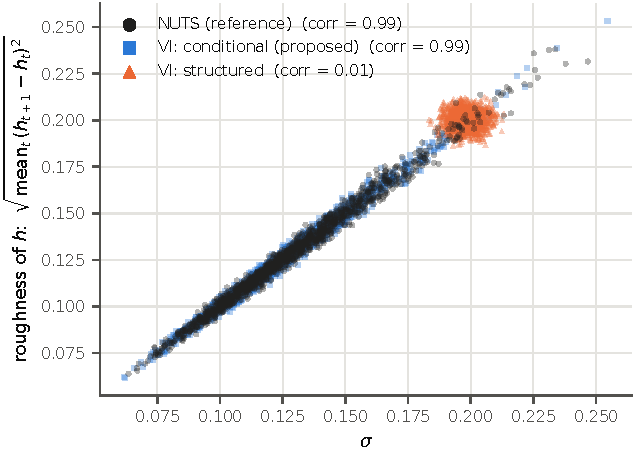
\includegraphics[width=0.75\linewidth]{figures/fig_sigma_roughness.pdf}
  \caption{$\sigma$ と $h$ の経路の粗さ $\sqrt{\mathrm{mean}_t (h_{t+1} - h_t)^2}$ の事後的な依存（一致度の実験の合成データ、高持続 $\phi = 0.99$、$\sigma = 0.10$、$T = 1{,}000$）。
    各点は事後分布（変分分布）からの 1 サンプル（各 1,500 点を表示）。括弧内は全サンプル（NUTS 16,000、VI 各 4,000）での相関係数。
    NUTS は 4 連鎖、ウォームアップ 2,000 の後に 32,000 回更新して 8 回に 1 回を保存。VI は 20,000 ステップ。}
  \label{fig:sigma-roughness}
\end{figure}

\subsection{条件付き構造化近似（提案）}\label{sec:fam-conditional}

構造化近似の問題は、$q(h)$ が $\theta$ に依存しないことにあった。
そこで、$h$ の変分分布を $\theta$ に条件付けた形にする。本稿では次の族を考え、\textbf{条件付き構造化変分族}と呼ぶ。
\begin{equation}
  q(u, h) = \Normal(u \mid m_u,\ C C^\top)\; q\!\left(h \mid \theta(u)\right), \qquad
  q(h \mid \theta) \;\propto\; p(h \mid \theta) \prod_{t=1}^{T} \Normal\!\left(\tilde y_t \;\middle|\; h_t,\ \lambda_t^{-1}\right).
  \label{eq:fam-conditional}
\end{equation}
$p(h \mid \theta)$ は SV モデルの AR(1) 事前分布そのもの、$\tilde y_t \in \mathbb{R}$ と $\lambda_t > 0$ は変分パラメータである。
$q(h \mid \theta)$ は、「AR(1) の事前分布を持つ $h$ について、$\tilde y_t$ という値を精度 $\lambda_t$ で観測したときの事後分布」という形をしている。
$\tilde y_t$ を\textbf{擬似観測}、$\lambda_t$ をその\textbf{精度}と呼ぶ。
真の観測 $y_t$ は $h_t$ について非線形・非正規な情報を与えるが（\cref{sec:model-likelihood}）、それを各日ごとの正規分布の形の情報で置き換えたもの、と見ることができる。
変分パラメータは $m_u$、$C$、$\tilde y_{1:T}$、$\log\lambda_{1:T}$ で、数は $k + k(k+1)/2 + 2T$ であり、構造化近似（$3T$ 程度）より少ない。

\paragraph{$q(h \mid \theta)$ の具体形}
\cref{eq:fam-conditional}の右辺の対数をとると、
\[
  \log q(h \mid \theta) = -\frac{1}{2}(h - \mu\mathbf{1})^\top Q_{\mathrm{AR}}(\phi, \sigma)\,(h - \mu\mathbf{1}) - \frac{1}{2}\sum_{t=1}^{T} \lambda_t (h_t - \tilde y_t)^2 + \text{定数}
\]
であり（$Q_{\mathrm{AR}}$ は\cref{eq:ar1-precision}の三重対角行列、$\mathbf{1}$ はすべて 1 のベクトル）、$h$ の二次式である。
したがって $q(h \mid \theta)$ は正規分布で、平方完成により
\begin{equation}
  \begin{gathered}
  q(h \mid \theta) = \Normal\!\left(h \;\middle|\; m(\theta),\ P(\theta)^{-1}\right), \\
  P(\theta) = Q_{\mathrm{AR}}(\phi, \sigma) + \diag(\lambda), \qquad
  m(\theta) = P(\theta)^{-1}\left( Q_{\mathrm{AR}}(\phi, \sigma)\, \mu\mathbf{1} + \lambda \odot \tilde y \right)
  \end{gathered}
  \label{eq:fam-conditional-gauss}
\end{equation}
を得る（$\odot$ は成分ごとの積）。
精度行列 $P(\theta)$ は三重対角行列に対角行列を足したものなので、やはり三重対角であり、構造化近似と同じく $O(T)$ で扱える。
平均は $m(\theta) = \mu\mathbf{1} + P(\theta)^{-1}\{\lambda \odot (\tilde y - \mu\mathbf{1})\}$ とも書ける。
擬似観測の情報（$\lambda$）が AR(1) の事前分布の精度に比べて小さい日には、$h_t$ の平均は長期水準 $\mu$ に引き寄せられ、大きい日には $\tilde y_t$ に近づく。

\paragraph{$\theta$ との依存}
この族では、$h$ の分布が $\theta$ の関数として自動的に変わる。
\begin{itemize}
  \item $\sigma$ が小さいと、$Q_{\mathrm{AR}}$ の成分（$\propto 1/\sigma^2$）が大きくなり、隣り合う $h_t$ を強く結びつける。
    すなわち $h$ の経路は\textbf{滑らかに}なり、平均も擬似観測の細かな変動を追わなくなる。$\sigma$ が大きければその逆である。
  \item $\mu$ が大きくなると、平均 $m(\theta)$ は事前分布の寄与の分だけ上に動く。
  \item $\phi$ が 1 に近づくと、遠く離れた日どうしの結びつきも強くなる。
\end{itemize}
これがまさに (R2) の依存である。
\cref{fig:sigma-roughness}のとおり、条件付き構造化近似は、$\sigma$ と経路の粗さの相関（0.99）と、両者の同時分布の形を NUTS とほぼ同じに再現している。

\paragraph{ラプラス近似との関係}
この族の形は、\cref{sec:model-structure}のラプラス近似から自然に導かれる。
$\theta$ を固定し、$h$ の事後分布の最頻値 $\hat h$ をニュートン法で求めることを考える。
各日の観測の対数尤度を現在の点 $\hat h_t$ のまわりで二次近似すると、
\[
  \log p(y_t \mid h_t) \approx \text{定数} + g_t (h_t - \hat h_t) - \frac{c_t}{2} (h_t - \hat h_t)^2
  = \text{定数} - \frac{c_t}{2}\left(h_t - \Bigl(\hat h_t + \frac{g_t}{c_t}\Bigr)\right)^2,
\]
\[
  g_t = -\frac{1}{2} + \frac{y_t^2}{2} e^{-\hat h_t}, \qquad c_t = \frac{y_t^2}{2} e^{-\hat h_t}
\]
となる（$g_t$、$c_t$ は 1 階・2 階微分の符号を変えたもの）。
これは「値 $\hat h_t + g_t / c_t$ を精度 $c_t$ で観測した」ときの対数尤度と同じ形であり、ニュートン法の各ステップは、AR(1) の事前分布とこの擬似観測による正規分布の事後分布を計算することに等しい。
ニュートン法が収束した点では、ラプラス近似の正規分布\cref{eq:laplace-precision}は、\cref{eq:fam-conditional-gauss}で $\tilde y_t = \hat h_t + g_t/c_t$、$\lambda_t = c_t$ としたものに一致する。
つまり条件付き構造化族は、\textbf{各 $\theta$ でのラプラス近似と同じ形の分布を、すべての $\theta$ について同時に表す族}である。
ただし擬似観測とその精度は $\theta$ によらない共通の値であり、それを（ラプラス近似のように最頻値から決めるのではなく）ELBO の最大化で決める。
擬似観測が $\theta$ によらないことはこの族の近似の一つであり、例えば $\theta$ によって擬似観測の最適な値が大きく変わる場合には誤差が生じる。

\paragraph{サンプリングとエントロピーの計算手順}
ELBO の推定値は、1 サンプルあたり次の手順で計算する（\code{advi.py} の \code{conditional\_factor} と \code{draw}）。
すべての手順が $O(T)$ であり、自動微分によって変分パラメータ全体についての勾配が得られる。
\begin{enumerate}[label=(\arabic*)]
  \item $\epsilon_u \sim \Normal(0, I_k)$ から $u = m_u + C\epsilon_u$ を作り、$\theta = \theta(u)$ に変換する。
  \item 三重対角行列 $P(\theta) = Q_{\mathrm{AR}}(\phi, \sigma) + \diag(\lambda)$ の対角 $a_t$ と副対角 $b_t$ を作る。
  \item コレスキー分解 $P(\theta) = L L^\top$ を漸化式
    $d_1 = \sqrt{a_1}$、$s_t = b_t / d_t$、$d_{t+1} = \sqrt{a_{t+1} - s_t^2}$
    で計算する（$L$ は下二重対角で、対角 $d_t$、副対角 $s_t$）。
  \item 平均 $m(\theta)$ を、$P(\theta) m = Q_{\mathrm{AR}}\mu\mathbf{1} + \lambda \odot \tilde y$ を前進代入（$L w = $ 右辺）と後退代入（$L^\top m = w$）で解いて求める。
  \item $\epsilon_h \sim \Normal(0, I_T)$ について $L^\top x = \epsilon_h$ を後退代入で解き、$h = m(\theta) + x$ とする。
  \item 対数同時密度\cref{eq:advi-jacobian}を $(u, h)$ で評価する。
\end{enumerate}
エントロピーは、同時分布のエントロピーの連鎖律
\[
  \mathcal{H}[q(u, h)] = \mathcal{H}[q(u)] + \E_{q(u)}\!\left[\mathcal{H}[q(h \mid \theta(u))]\right], \qquad
  \mathcal{H}[q(h \mid \theta)] = \frac{T}{2}(1 + \log 2\pi) - \sum_{t=1}^{T} \log d_t(\theta)
\]
で計算する。第 1 項は $q(u)$ が正規分布なので解析的に書け、第 2 項の期待値は (1) で引いた $M$ 個の $u$ での標本平均で推定する（不偏推定）。
第 2 項の中の $d_t(\theta)$ は (3) で計算済みなので、追加の計算はほとんどない。
こうして $M = 4$ 個のサンプルで ELBO を推定し、その勾配で Adam の 1 ステップを進める。
1 ステップの計算は、$M$ 本の長さ $T$ の漸化式（\code{jax.lax.scan}）を数回回すことに相当する。

\paragraph{パラメータ化に依存しないこと}
非中心化パラメータ化（$x = (h - \mu)/\sigma$）で同じ族を使う場合は、上の手順で $h$ を作ったあと $x = (h - \mu)/\sigma$ と変換する。
$\theta$ を固定すれば、これは $h$ のアフィン変換なので、$x$ の分布も三重対角の精度行列を持つ正規分布であり、エントロピーは $T\log\sigma$ だけ減る（実装ではこの補正を入れている）。
このとき $(\theta, h)$ の同時分布としては、中心化で作った $q$ とまったく同じ分布族になる。
ELBO は未知数の可逆な変数変換によって変わらない（$\log p$ と $\log q$ が同じヤコビアンの分だけ変わり、打ち消し合う）ので、
\textbf{条件付き構造化族では、中心化・非中心化のどちらを使っても同じ最適解と同じ ELBO が得られる}。
これに対して、平均場・構造化・フルランクの族では、$h$ に正規分布を当てるか $x$ に当てるかで $(\theta, h)$ の同時分布の族そのものが変わる（$h = \mu + \sigma x$ は $\theta$ と $x$ について非線形なので）。
例えば非中心化の構造化族では、$h$ の広がりが $\sigma$ に比例して変わるので (R2) の依存の一部が表せるようになり、$\sigma$ の不確実性の過小評価が緩和される（\cref{app:settings}）。
条件付き構造化族は、そうした依存を最初から族に組み込んでいるので、パラメータ化を選ぶ必要がない（R4）。
この性質は数値的にも確認しており、中心化と非中心化で推定結果は一致する（\cref{app:settings}）。

\paragraph{位置付け}
条件付き構造化族は、\cref{sec:intro-related}で述べた既存の考え方の組み合わせである。
局所変数（ここでは $h$）の変分分布を大域パラメータに条件付けるという構造は \textcite{tan2020} と同じであり、
「事前分布 × 正規分布の擬似観測」という表現は、\textcite{johnson2016} が状態空間モデルの構造化 VI でニューラルネットワークに出力させた共役な因子を、自由な変分パラメータで置き換えたものにあたる。
また \textcite{loaizamaya2022} は、潜在変数について近似ではなく正確な条件付き事後分布 $p(h \mid y, \theta)$ を使う族を提案しているが、
SV モデルでは $p(h \mid y, \theta)$ からの正確なサンプリング自体に MCMC などが必要になる。
本稿の族は、その代わりに $\theta$ ごとのラプラス近似と同じ形の正規分布を使うことで、すべての計算を閉じた形・$O(T)$ に保っている。
手法としての新しさよりも、SV モデルの構造（AR(1) 事前分布の三重対角の精度行列と、$\sigma$ が滑らかさを決めるという依存）を変分族に正しく入れることの効果を示すことが、本稿の主眼である。

\subsection{レバレッジ SV への拡張}\label{sec:fam-leverage}

レバレッジ SV では、$\theta$ を固定したときの $h$ の事後分布の形が変わる。
\cref{eq:sv-leverage-state}を使うと、同時分布は
\[
  p(y, h \mid \theta) = p(h_1 \mid \theta) \prod_{t=1}^{T-1} p(h_{t+1} \mid h_t, y_t, \theta) \prod_{t=1}^{T} p(y_t \mid h_t)
\]
と分解できる（$y_t$ の周辺分布 $p(y_t \mid h_t)$ は $\Normal(0, e^{h_t})$ のまま）。
$h$ の事後分布の「事前分布にあたる部分」は、もはや $p(h \mid \theta)$ ではなく、
イノベーションの分散が $\sigma^2(1 - \rho^2)$ に縮み、平均に $\rho\sigma\, y_t e^{-h_t/2}$ というリターンに連動したドリフトが加わった遷移 $p(h_{t+1} \mid h_t, y_t, \theta)$ の積になる。

基本 SV の族をそのまま使い、$q(h \mid \theta)$ を $\rho$ によらない AR(1) 事前分布から作ると、$\rho$ と $h$ の依存がまったく表せない。
本稿の予備実験では、この最初の版は $\rho$ の推定値をほぼ 0（$-0.08$。真値 $-0.5$）に潰してしまった。
第 3 章で見た平均場の $\phi$ と同じ理屈で、ELBO が「$q$ の近似が正確になる $\rho = 0$」を好んだためと考えられる。

そこで、$q(h \mid \theta)$ の遷移部分をレバレッジ SV の遷移に合わせて
\begin{equation}
  \begin{aligned}
  q(h \mid \theta) \;\propto\;& \Normal\!\left(h_1 \;\middle|\; \mu, \frac{\sigma^2}{1-\phi^2}\right)
    \prod_{t=1}^{T-1} \Normal\!\left(h_{t+1} \;\middle|\; \mu + \phi(h_t - \mu) + \rho\sigma\,\tilde e_t,\ \sigma^2(1 - \rho^2)\right) \\
    &\times \prod_{t=1}^{T} \Normal\!\left(\tilde y_t \;\middle|\; h_t, \lambda_t^{-1}\right)
  \end{aligned}
  \label{eq:fam-leverage}
\end{equation}
とする。真のドリフトの中の標準化リターン $y_t e^{-h_t/2}$ を、新たな変分パラメータ $\tilde e_t$（$t = 1, \dots, T-1$）で置き換えたものである。
こうすると $q(h \mid \theta)$ は再び正規分布になり、精度行列はイノベーションの標準偏差を $\sigma\sqrt{1 - \rho^2}$ とした AR(1) の精度行列に $\diag(\lambda)$ を足した三重対角行列、
平均の計算ではドリフト $\rho\sigma\tilde e_t$ が右辺の 1 次の項に加わるだけで、計算はすべて $O(T)$ のまま変わらない。
$\rho$ が変わると、$h$ の遷移の不確実性（$\sigma^2(1 - \rho^2)$）とドリフトの大きさ（$\rho\sigma\tilde e_t$）が連動して変わるので、$\rho$ と $h$ の依存の主要な部分が表せる。
この修正により、予備実験の $\rho$ の推定値は $-0.37$ まで改善した。

それでも、合成データの復元実験では、$\rho$ は真値より 0 の側に約 25\% 縮んで推定される（$T = 2{,}000$ で偏り $+0.13$、95\% 区間の被覆率 0.35、事後標準偏差は NUTS の 0.65 倍。\cref{sec:synthetic}）。
残る偏りの原因は、真のドリフト $\rho\sigma\, y_t e^{-h_t/2}$ が $e^{-h_t/2}$ を通じて $h_t$ に\textbf{非線形に}依存することにある。
$h_t$ が高い日ほど同じリターンでも標準化リターンは小さく、ドリフトも小さくなるが、$\tilde e_t$ を $h_t$ によらない定数とした正規分布の族ではこの依存が表せない。
ステップ数や学習率を変えても偏りは変わらなかったので、最適化の問題ではなく族の表現力の限界である。
これを解消するには、遷移が $h_t$ に非線形に依存する変分族（例えば正規化フロー）が必要になり、今後の課題とする（\cref{sec:conclusion}）。
なお実データでは、$\rho$ の推定値の差は NUTS との比較で 0.02〜0.06 程度であった（\cref{sec:empirical}）。

実装上の注意として、$\tilde e_t$ の初期値を 0 にしてはならない。
ドリフトは $\rho\sigma\tilde e_t$ という積の形をしているので、$\rho$ についての勾配は $\tilde e_t$ に比例し、$\tilde e_t$ についての勾配は $\rho$ に比例する。
$\rho$ の初期値は 0 なので、$\tilde e_t$ も 0 から始めると両方の勾配が 0 になり、最適化がそこから動かない（鞍点）。
本稿では、$\tilde e_t$ の初期値を、$h$ の初期値 $h^{(0)}_t$ による標準化リターン $y_t e^{-h^{(0)}_t/2}$ とした。

\subsection{\texorpdfstring{$t$}{t} 誤差の SV への適用}\label{sec:fam-t}

$t$ 誤差の SV モデルでは、状態方程式は基本 SV と同じであり、観測の尤度だけが変わる。
条件付き構造化族の $q(h \mid \theta)$ は、事前分布の部分（$p(h \mid \theta)$）と擬似観測の部分からなり、観測の尤度の形は擬似観測が吸収するので、族の形を変える必要はない。
自由度 $\nu$ は大域パラメータとして $u$ に加え（$\nu = 2 + e^{u_\nu}$）、$q(u)$ を 4 次元のフルランクの正規分布にするだけである。
$t$ 分布の対数尤度は $h_t$ についての曲率に上限がある（\cref{sec:model-likelihood}）ので、極端なリターンの日には最適な擬似観測の精度 $\lambda_t$ が小さくなり、その日の観測の影響が自動的に弱まると期待される。

\subsection{変分族の比較}\label{sec:fam-summary}

\cref{tab:families}に、本稿で比較する変分族の性質をまとめる。
パラメータ数は、基本 SV（$k = 3$）、$T = 1{,}000$ のときに実際に最適化される変分パラメータの数である（下三角行列は $k(k+1)/2$ 個と数える）。
条件付き構造化族は、本稿で比較する族の中で (R1)〜(R4) のすべてを満たす唯一の族であり、しかもパラメータ数は平均場とほとんど変わらない。
その違いを生んでいるのは、パラメータの数ではなく、モデルの構造（AR(1) の事前分布）を変分族の中にそのまま組み込んでいることである。

\begin{table}[tbp]
  \centering
  \caption{変分族の比較（基本 SV、$T = 1{,}000$）。
    (R1)〜(R4) は\cref{sec:fam-requirements}の要件で、○は満たす、△は一部のみ、×は満たさない。
    (R1) は $h_t$ の時間方向の相関、(R2) は $\theta$ と $h$ の依存（フルランクは正規分布で表せる線形の依存のみ、低ランクは少数の因子を通じた依存のみ）、
    (R3) の計算量は 1 サンプルあたりのサンプリングと密度計算の計算量、パラメータ数は実際に最適化される変分パラメータの数（下三角行列は $k(k+1)/2$ 個と数える）、
    (R4) の不変性は中心化と非中心化で $(\theta, h)$ の分布の族が変わらないこと。}
  \label{tab:families}
  \footnotesize
  \setlength{\tabcolsep}{4pt}
  \begin{tabular}{lllcccrc}
\toprule
 & \multicolumn{2}{c}{共分散（精度）の構造} & (R1) & (R2) & \multicolumn{2}{c}{(R3)} & (R4) \\
\cmidrule(lr){2-3} \cmidrule(lr){6-7}
変分族 & $q(\theta)$ & $q(h)$ & 時間相関 & $\theta$--$h$ 依存 & 計算量 & パラメータ数 & 不変性 \\
\midrule
平均場 & 対角 & 対角 & × & × & $O(T)$ & 2,006 & × \\
低ランク（$r=10$） & \multicolumn{2}{c}{$WW^\top + D$} & △ & △ & $O(Tr)$ & 12,036 & × \\
フルランク & \multicolumn{2}{c}{密な共分散 $LL^\top$} & ○ & △ & $O(T^2)$ & 504,509 & × \\
構造化 & フルランク & 三重対角の精度 & ○ & × & $O(T)$ & 3,008 & × \\
条件付き構造化 & フルランク & $Q_{\mathrm{AR}}(\theta) + \diag(\lambda)$ & ○ & ○ & $O(T)$ & 2,009 & ○ \\
\bottomrule
\end{tabular}

\end{table}

\subsection{初期値}\label{sec:fam-init}

VI は最適化なので、初期値が結果や収束の速さに影響しうる。
本稿では、すべての手法（NUTS を含む）で共通の初期値を使う（\code{initialization.py}）。
\begin{itemize}
  \item \textbf{$h$ の初期値}：$\log y_t^2 = h_t + \log\varepsilon_t^2$ と $\E[\log\varepsilon_t^2] \approx -1.27$（\cref{sec:model-likelihood}）から、
    $h^{(0)}_t$ を $\log(y_t^2 + c) + 1.27$ の 10 日移動平均とする。$c = 0.1 \times \overline{y^2}$ は、リターンが 0 の日に対数が発散するのを防ぐための小さな定数である。
  \item \textbf{$\theta$ の初期値}：$\phi = 0.95$、$\sigma = 0.2$、$\mu = h^{(0)}$ の平均、レバレッジ SV では $\rho = 0$、$t$ 誤差の SV では $\nu = 10$。
    NUTS では、これを無制約空間で連鎖ごとに標準偏差 0.1 だけずらして使う（\cref{sec:inf-mcmc}）。
\end{itemize}
変分パラメータの初期値は、族ごとに次のように決める（\code{advi.py} の \code{init\_params}）。
\begin{itemize}
  \item \textbf{$q(u)$}（構造化・条件付き構造化）：平均は $\theta$ の初期値を無制約空間に写したもの、$C = 0.1\, I$。
  \item \textbf{平均場}：$h$ の平均は $h^{(0)}$、標準偏差は $1/\sqrt{\Lambda_{tt}}$（$\Lambda = Q_{\mathrm{AR}}(\theta^{(0)}) + \frac{1}{2}I$）。これは正規分布の目標に対する平均場の最適解（\cref{sec:inf-vi}）である。大域パラメータの標準偏差は 0.1。
  \item \textbf{構造化}：$m_h = h^{(0)}$、$L$ は $Q_{\mathrm{AR}}(\theta^{(0)}) + \frac{1}{2}I$ のコレスキー因子。
  \item \textbf{条件付き構造化}：$\tilde y_t = h^{(0)}_t$、$\lambda_t = 1/2$、レバレッジ SV では $\tilde e_t = y_t e^{-h^{(0)}_t/2}$。
\end{itemize}
ここで 1/2 は、観測 1 つが $h_t$ について持つ期待フィッシャー情報 $\E[y_t^2 e^{-h_t}]/2 = 1/2$ である（\cref{sec:inf-vi}）。
つまり、精度の初期値は「$\theta^{(0)}$ でのラプラス近似」を大まかに真似たものになっている。
初期値への感度は\cref{app:settings}で確認している。

時点ごとの変分パラメータ（$\tilde y_t$、$\lambda_t$、$\tilde e_t$ など）は、推定期間を 1 日ずらしたときに 1 つずらして次の日の初期値に使える。
これを使った日次の再推定（warm start）は\cref{sec:system}で扱う。

% 5 章：合成データによる検証（実験 S1〜S4）
% 数値は results/s1〜s4 の CSV から（memo/09_results_synthetic.md に要約）。
% 表は experiments/s1_recovery.py（tab1_recovery・tab1b_leverage・tab1c_student_t）、s2_agreement.py（tabA2_agreement）、
% s3_scaling.py（tabA3_scaling）、s4_sensitivity.py（tabA1_sensitivity）が生成。図は同じスクリプトが生成（fig2〜fig4、figA1）。
% 付録に回す予定の図表（図A1、表A1〜A3）も、分量の調整までは本章に置いている。
\section{合成データによる検証}\label{sec:synthetic}

本章では、真のパラメータと真のボラティリティが分かっている合成データを使って、\cref{sec:family}の変分族を評価する。
実データでは「正解」が分からないため、推定方法そのものの良し悪しは、まず合成データで確かめておく必要がある。
\cref{sec:syn-overview}で実験の全体像を、\cref{sec:syn-setup}で共通の設定と評価指標を述べる。
\cref{sec:syn-recovery,sec:syn-agreement,sec:syn-scaling,sec:syn-sensitivity}で四つの実験の結果を順に示し、
\cref{sec:syn-summary}で本章の結果をまとめる。

\subsection{実験の目的と全体像}\label{sec:syn-overview}

本章の実験は、次の四つの問いに答えるために設計した。

\begin{enumerate}[label=(Q\arabic*)]
  \item \textbf{真値をどれだけ正確に復元できるか}（実験 S1）。
    多数の合成データについて、パラメータ $\theta$ と潜在ボラティリティ $h_{1:T}$ の推定値が真値にどれだけ近いか、
    95\% 信用区間が名目どおり真値を含むかを調べる。
  \item \textbf{NUTS の事後分布にどれだけ一致するか}（実験 S2）。
    1 本のデータについて、十分に長く回した NUTS を「正解」とし、VI の事後分布の位置と広がりを比べる。
    S1 が「真値との比較」であるのに対し、S2 は「正確なベイズ推定との比較」であり、近似の質そのものを測る。
  \item \textbf{計算時間は系列長 $T$ とともにどう伸びるか}（実験 S3）。
    $T$ を 250 から 10,000 まで変えて、NUTS と VI の所要時間を測る。
  \item \textbf{結果は設定に左右されないか}（実験 S4）。
    パラメータ化（中心化・非中心化）、$\sigma$ の事前分布、ELBO のモンテカルロ（MC）サンプル数、学習率を変えて、推定値が変わるかを調べる。
\end{enumerate}

\cref{tab:syn-design}に各実験の設計をまとめる。
比較する手法は、正解役の NUTS と、\cref{sec:family}の三つの変分族（平均場、構造化、条件付き構造化）を自前の ADVI で最適化したものである。
低ランク・フルランクの族は、\cref{sec:fam-dense}で述べたとおり平均場と同様に崩れるため、S2 で NumPyro の実装を参考として併記するにとどめる。

\begin{table}[tbp]
  \centering
  \caption{合成データ実験の設計。}
  \label{tab:syn-design}
  \footnotesize
  \begin{tabular}{>{\raggedright\arraybackslash}p{0.12\linewidth}>{\raggedright\arraybackslash}p{0.25\linewidth}>{\raggedright\arraybackslash}p{0.24\linewidth}>{\raggedright\arraybackslash}p{0.25\linewidth}}
    \toprule
    実験 & データ & 手法 & 主な評価指標 \\
    \midrule
    S1 復元精度 & 5 シナリオ × $T \in \{500, 2{,}000\}$ × 各 20 本（計 200 本） & NUTS、条件付き構造化（提案）、構造化、平均場 & $\theta$ の偏り・RMSE・95\% 区間の被覆率、$h$ の RMSE・被覆率・sd 比、計算時間 \\
    \addlinespace
    S2 NUTS との一致度 & 高持続シナリオ、$T = 1{,}000$、1 本 & S1 の 4 手法 ＋ NumPyro の 4 ガイド（構造化・平均場・低ランク・フルランク）。NUTS は長い連鎖 & 事後平均、sd 比、Wasserstein 距離、ELBO、$\hat k$、計算時間 \\
    \addlinespace
    S3 計算時間 & 標準シナリオ、$T = 250$〜$10{,}000$ の 6 通り、各 1 本 & NUTS、提案、構造化、平均場（自前・NumPyro） & 所要時間、NUTS の最小 ESS・最大 $\hat R$ \\
    \addlinespace
    S4 設定への感度 & 高持続シナリオ、$T = 1{,}000$、5 本 & 3 族 × 中心化・非中心化、提案手法の事前分布・MC サンプル数・学習率 & 事後平均、NUTS に対する sd 比、収束ステップ \\
    \bottomrule
  \end{tabular}
\end{table}

\subsection{実験設定}\label{sec:syn-setup}

\subsubsection{シナリオとデータの生成}

合成データは、\cref{sec:model}のモデルから直接生成する。
基本 SV モデルについては、持続性の異なる三つのシナリオを用意した。

\begin{itemize}
  \item \textbf{標準}：$\mu = 0$、$\phi = 0.97$、$\sigma = 0.15$。
    日次の株価指数に SV モデルを当てはめたときの典型的な値で、ボラティリティショックの半減期は約 23 日である。
  \item \textbf{高持続}：$\mu = 0$、$\phi = 0.99$、$\sigma = 0.10$。
    ボラティリティの局面が長く続く（半減期は約 69 日）ケースで、隣り合う日の $h_t$ の事後相関がもっとも強い。
    \cref{tab:meanfield-gap}で見たとおり、平均場近似にとってもっとも厳しい設定である。
  \item \textbf{低持続}：$\mu = 0$、$\phi = 0.80$、$\sigma = 0.40$。
    ボラティリティが速く平均に戻る（半減期は約 3 日）ケースである。
    本稿の実データ（1321・1306）の NUTS による推定値は $\phi \approx 0.86$〜$0.89$、$\sigma \approx 0.38$〜$0.46$ であり（\cref{tab:sv-properties}）、
    取得できた期間が約 2 年と短いこともあって、標準シナリオよりもこの低持続シナリオに近い。
\end{itemize}

三つのシナリオは、$h_t$ の定常分布の標準偏差 $s = \sigma / \sqrt{1 - \phi^2}$ がほぼ同じ（0.62〜0.71）になるように選んでいる。
そのため、リターンの尖度や年率ボラティリティの変動幅（\cref{tab:sv-properties}）はシナリオ間でほぼ同じで、違いはボラティリティの「動きの速さ」だけである。
これにより、変分族の性能が持続性 $\phi$ にどう依存するかを、他の要因と切り分けて調べられる。

拡張モデルについては、標準シナリオのパラメータに一つずつ要素を加えた二つのシナリオを用意した。

\begin{itemize}
  \item \textbf{レバレッジ}：標準シナリオに $\rho = -0.5$ を加える（\cref{sec:model-leverage}）。
    日次の株価指数の推定値としてよく報告される水準である。
  \item \textbf{$t$ 誤差}：標準シナリオの誤差を、自由度 $\nu = 8$ の標準化 $t$ 分布にする（\cref{sec:model-t}）。
\end{itemize}

いずれのシナリオでも、$h_1$ は定常分布 $\Normal(\mu, s^2)$ から生成し、その後は\cref{eq:sv-state}に従って $h_2, \dots, h_T$ を生成し、\cref{eq:sv-obs}からリターン $y_t$（\% 単位）を作る。
$\mu = 0$ なので、日次ボラティリティの水準は 1\% 程度（年率で約 16\%）である。
真の平均が 0 のデータなので、実データ（\cref{sec:model-data}）のような標本平均の除去は行わない。
乱数のシードは、実験の番号・シナリオ・$T$・複製の番号から決定的に作り、すべての結果を再現できるようにしている。

\subsubsection{手法の設定}

事前分布は全実験で\cref{tab:priors}の標準の設定を使う（S4 の $\sigma$ の事前分布の比較を除く）。
推定はすべて中心化パラメータ化で行う（S4 のパラメータ化の比較を除く）。
初期値は全手法で共通で、\cref{sec:fam-init}の方法で作る。

\paragraph{NUTS}
NumPyro の NUTS を 4 連鎖で実行する。目標受理率は 0.9 とし、各連鎖の初期値は共通の初期値に小さな乱数（無制約空間で標準偏差 0.1）を加えてずらす。
4 連鎖は CPU の 4 コアで並列に実行する。反復数は実験ごとに次のように変えた。

\begin{itemize}
  \item S1・S4：ウォームアップ 2,000 回、サンプリング 2,000 回（各連鎖。合計 8,000 サンプル）。
    200 本ものデータを推定するため、計算時間と精度の折り合いをつけた長さである。
  \item S2：ウォームアップ 2,000 回の後、32,000 回更新して 8 回に 1 回を保存（各連鎖 4,000 サンプル、合計 16,000 サンプル）。
    VI を評価する「正解」として使うため、十分に長くした。
  \item S3：ウォームアップ 1,000 回、サンプリング 1,000 回。
    実務で「とりあえず回す」ときの長さを想定した。
\end{itemize}

\paragraph{VI}
三つの変分族とも、\cref{sec:inf-advi}の ADVI で最適化する。
最適化手法は Adam で、学習率は 0.01 から始めて最後に 0.001 になるよう指数的に下げる。
ELBO の勾配は、1 ステップあたり $M = 4$ 個の MC サンプルで推定する。
ステップ数は S1・S3・S4 で 10,000、S2 で 20,000 とし、収束したかどうかにかかわらず決められた回数だけ回す（\cref{sec:inf-diagnostics}）。
最適化の後、変分分布から 1,000 個のサンプルを引いて、事後平均や 95\% 区間を計算する。
S2 では、NumPyro の SVI で、平均場（\code{AutoNormal}）、低ランク（\code{AutoLowRankMultivariateNormal}、ランク 10）、
フルランク（\code{AutoMultivariateNormal}）、構造化（自作のガイド）の 4 つも同じステップ数・学習率で最適化した。

\subsubsection{評価指標}

\paragraph{パラメータ}
シナリオ・$T$ ごとに $R$ 本（S1 では $R = 20$）の複製データがあり、$r$ 本目のデータに対する手法の事後平均を $\hat\theta^{(r)}$、
95\% 信用区間（事後分布の 2.5\% 点と 97.5\% 点）を $[\ell^{(r)}, u^{(r)}]$ とする。真値を $\theta^\ast$ とすると、
\begin{equation}
  \begin{gathered}
    \text{偏り} = \frac{1}{R}\sum_{r=1}^R (\hat\theta^{(r)} - \theta^\ast), \qquad
    \mathrm{RMSE} = \sqrt{\frac{1}{R}\sum_{r=1}^R (\hat\theta^{(r)} - \theta^\ast)^2}, \\
    \text{被覆率} = \frac{1}{R}\sum_{r=1}^R \mathbb{1}\{\ell^{(r)} \le \theta^\ast \le u^{(r)}\}
  \end{gathered}
  \label{eq:syn-metrics}
\end{equation}
である。
被覆率は、区間の幅が適切かどうかを測る指標で、名目の 95\% に近いことが望ましい。
被覆率が名目を大きく下回るのは、区間が狭すぎる（不確実性の過小評価）か、区間の位置がずれている（推定の偏り）かのどちらかである。

\paragraph{潜在ボラティリティ}
$h_{1:T}$ については、時点ごとの事後平均の RMSE $\sqrt{T^{-1}\sum_t (\hat h_t - h_t^\ast)^2}$ と、
時点ごとの 95\% 区間が真値を含む割合（時点についての平均）を、データごとに計算して複製で平均する。

注意したいのは、$h_t$ の RMSE は、事後分布を正確に計算できたとしても 0 にはならない点である。
1 日の観測 $y_t$ が $h_t$ について持つ情報は少なく（\cref{sec:model-structure}）、事後分布にはもともと幅がある。
本章の実験では、NUTS でも $h_t$ の RMSE は 0.27（高持続）〜0.53（低持続）である。
このため、$h_t$ の RMSE だけでは手法の差が見えにくく、事後分布の広がりが正しいかを別に調べる必要がある。

\paragraph{NUTS との比較}
VI の事後分布の広がりが正しいかは、NUTS の事後標準偏差との比（\textbf{sd 比}）$\mathrm{sd}_{\mathrm{VI}} / \mathrm{sd}_{\mathrm{NUTS}}$ で測る。
1 なら NUTS と同じ広がり、1 未満なら VI が不確実性を過小評価、1 より大きければ過大評価していることになる。
$h$ については、時点ごとの sd 比の中央値を使う。
S1 では、データごとに sd 比を計算し、複製についての中央値を報告する。

S2 では、さらに次の二つを使う。
一つは、パラメータごとの周辺事後分布の \textbf{1 次元 Wasserstein 距離}で、VI と NUTS のサンプルの分布がどれだけ離れているかを、パラメータと同じ単位で測る。
もう一つは、$h_t$ の\textbf{基準化した平均差} $|\hat h_t^{\mathrm{VI}} - \hat h_t^{\mathrm{NUTS}}| / \mathrm{sd}_{\mathrm{NUTS}}(h_t)$ の時点についての中央値で、
VI の事後平均が NUTS の事後平均から、NUTS の事後標準偏差の何倍ずれているかを表す。
また、ELBO の値（最後の 500 ステップの平均）と PSIS の $\hat k$（\cref{sec:inf-diagnostics}）も報告する。

\paragraph{計算時間}
計算時間は、実行開始から結果が出るまでの経過時間（wall-clock）で測り、JAX の JIT コンパイルの時間を含める。
VI については、二つの時間を区別する。
一つは、決められたステップ数（S1・S3 では 10,000）をすべて実行するのにかかった\textbf{総時間}である。
もう一つは、\textbf{ELBO が収束するまでの時間}で、コンパイル時間に、実行時間を「収束したステップ ÷ 総ステップ数」の割合で按分したものを加えて求める。
収束したステップは、\cref{sec:inf-diagnostics}の判定（200 ステップごとの ELBO の平均の相対変化が $10^{-4}$ を下回った最初の時点）で決める。
前者は「いまの実装で実際にかかった時間」、後者は「収束したところで止めれば、どこまで短くできるか」の目安である。

\paragraph{被覆率の読み方}
S1 の被覆率は 20 本の複製から計算するため、1 本で 0.05 ずつしか変わらない。
真の被覆確率が 0.95 であっても、20 本中の被覆数は二項分布に従ってばらつき、被覆率の標準誤差は $\sqrt{0.95 \times 0.05 / 20} \approx 0.05$ になる。
したがって、0.85〜1.00 程度の被覆率は「名目どおり」と区別できない。
本章で問題にするのは、被覆率が 0.5 を下回るような、統計的なばらつきでは説明できない大きな外れである。

\subsubsection{計算環境}
計算はすべて 1 台のマシン（CPU 12 コア、WSL2 上の Linux、GPU なし）で行った。
ソフトウェアは Python 3.12、JAX 0.12、NumPyro 0.22 で、計算はすべて倍精度（float64）で行う。
VI の最適化は 1 プロセスで実行し、NUTS の 4 連鎖は 4 つの CPU デバイスで並列に実行する。
計時の公平のため、S3 はほかの重い処理と同時に走らせないようにした。

\subsection{真値の復元精度（S1）}\label{sec:syn-recovery}

\cref{tab:recovery}に、基本 SV モデルの三つのシナリオでの結果を示す。
5 シナリオ × 2 通りの $T$ × 20 本 = 200 本のデータを、4 つの手法で推定した（総計算時間は約 5.5 時間）。
表には $\phi$ と $\sigma$ の結果を載せ、$\mu$ については本文で触れる。

\begin{table}[tbp]
  \centering
  \caption{真値の復元精度（S1、基本 SV モデル、各条件 20 本の複製）。
    RMSE と被覆率（95\% 信用区間が真値を含む割合）は\cref{eq:syn-metrics}。
    $h_t$ の RMSE と被覆率は時点について平均したもので、複製で平均している。
    sd 比は、$h_t$ の事後標準偏差の NUTS に対する比（時点についての中央値）の、複製についての中央値。
    時間は JIT コンパイルを含む総時間の中央値（VI は 10,000 ステップ、NUTS は 4 連鎖でウォームアップ・サンプリング各 2,000 回）。}
  \label{tab:recovery}
  \small
  \setlength{\tabcolsep}{4pt}
  \begin{tabular}{llrrrrrrrr}
\toprule
 & & \multicolumn{2}{c}{$\phi$} & \multicolumn{2}{c}{$\sigma$} & \multicolumn{3}{c}{$h_t$} & \\
$T$ & 手法 & RMSE & 被覆 & RMSE & 被覆 & RMSE & 被覆 & sd比 & 時間[s] \\
\midrule
\multicolumn{10}{l}{標準 ($\phi=0.97$)} \\
500 & NUTS (reference) & 0.058 & 0.90 & 0.066 & 0.90 & 0.333 & 0.96 & -- & 11.5 \\
 & VI: conditional (proposed) & 0.054 & 0.85 & 0.054 & 0.90 & 0.332 & 0.95 & 0.95 & 3.2 \\
 & VI: structured & 0.056 & 0.05 & 0.060 & 0.00 & 0.331 & 0.97 & 1.01 & 1.9 \\
 & VI: mean-field & 0.906 & 0.00 & 0.388 & 0.00 & 0.504 & 0.92 & 1.33 & 5.9 \\
2000 & NUTS (reference) & 0.016 & 0.90 & 0.027 & 0.95 & 0.327 & 0.96 & -- & 47.2 \\
 & VI: conditional (proposed) & 0.013 & 0.85 & 0.022 & 0.95 & 0.327 & 0.95 & 0.96 & 11.9 \\
 & VI: structured & 0.028 & 0.10 & 0.057 & 0.00 & 0.333 & 0.97 & 1.09 & 7.3 \\
 & VI: mean-field & 0.938 & 0.00 & 0.399 & 0.00 & 0.559 & 0.92 & 1.46 & 18.6 \\
\midrule
\multicolumn{10}{l}{高持続 ($\phi=0.99$)} \\
500 & NUTS (reference) & 0.045 & 0.90 & 0.064 & 0.80 & 0.270 & 0.98 & -- & 13.4 \\
 & VI: conditional (proposed) & 0.041 & 0.75 & 0.054 & 0.85 & 0.268 & 0.97 & 0.96 & 3.3 \\
 & VI: structured & 0.050 & 0.05 & 0.103 & 0.00 & 0.285 & 0.99 & 1.19 & 1.9 \\
 & VI: mean-field & 0.903 & 0.00 & 0.540 & 0.00 & 0.541 & 0.93 & 1.49 & 5.8 \\
2000 & NUTS (reference) & 0.007 & 0.95 & 0.020 & 0.95 & 0.268 & 0.96 & -- & 73.3 \\
 & VI: conditional (proposed) & 0.006 & 0.85 & 0.017 & 0.95 & 0.268 & 0.95 & 0.97 & 11.9 \\
 & VI: structured & 0.035 & 0.00 & 0.100 & 0.00 & 0.290 & 0.99 & 1.40 & 7.4 \\
 & VI: mean-field & 0.951 & 0.00 & 0.490 & 0.00 & 0.598 & 0.91 & 1.83 & 18.5 \\
\midrule
\multicolumn{10}{l}{低持続 ($\phi=0.80$)} \\
500 & NUTS (reference) & 0.055 & 0.95 & 0.069 & 1.00 & 0.535 & 0.95 & -- & 7.2 \\
 & VI: conditional (proposed) & 0.056 & 0.90 & 0.070 & 1.00 & 0.536 & 0.92 & 0.94 & 3.1 \\
 & VI: structured & 0.107 & 0.00 & 0.166 & 0.00 & 0.545 & 0.84 & 0.75 & 1.9 \\
 & VI: mean-field & 0.721 & 0.00 & 0.273 & 0.00 & 0.613 & 0.93 & 1.10 & 5.7 \\
2000 & NUTS (reference) & 0.036 & 1.00 & 0.046 & 0.95 & 0.521 & 0.94 & -- & 21.2 \\
 & VI: conditional (proposed) & 0.036 & 0.90 & 0.058 & 0.95 & 0.522 & 0.92 & 0.93 & 11.5 \\
 & VI: structured & 0.102 & 0.00 & 0.174 & 0.00 & 0.540 & 0.84 & 0.75 & 7.2 \\
 & VI: mean-field & 0.769 & 0.00 & 0.181 & 0.00 & 0.617 & 0.90 & 1.00 & 18.2 \\
\bottomrule
\end{tabular}

\end{table}

\subsubsection{平均場：持続性 $\phi$ が崩れる}

平均場 VI は、すべてのシナリオ・系列長で $\phi$ の推定に失敗した。
$\phi$ の事後平均は、真値 0.80〜0.99 に対して 20 本の平均で 0.03〜0.09 にとどまり（個々のデータでも最大 0.39）、
RMSE は 0.72〜0.95、被覆率は 0 である。
$T$ を 500 から 2,000 に増やしても改善しない。
これは、\cref{sec:inf-vi}で説明したように、$\phi$ が大きいほど平均場近似の KL の最小値が大きくなり、ELBO が小さい $\phi$ を好むためである。
データを増やしても、$\log p(y \mid \theta)$ と KL の最小値はどちらも $T$ にほぼ比例して増えるので、この偏りは消えない。

$\phi$ が崩れると、ほかのパラメータも引きずられる。
$\phi \approx 0$ の AR(1) では、$h_t$ の日々の変動はすべて $\sigma$ が担うことになるため、$\sigma$ は真値の 0.10〜0.40 に対して 0.52〜0.65 に大きく推定される（偏り $+0.17$〜$+0.50$）。
$h_t$ は日ごとにほぼ独立に推定されるので、ボラティリティの推定値は日々のリターンの大きさに引きずられて激しく上下し、
$h_t$ の RMSE は NUTS の 1.1〜2.2 倍（0.50〜0.62）に悪化する。

注目すべきは、$h_t$ の事後標準偏差がむしろ NUTS の 1.0〜1.8 倍に\textbf{広がっている}ことである。
「平均場近似は事後分散を過小評価する」という一般的な理解（\cref{sec:inf-vi}）とは逆の現れ方であるが、
これは、$\phi$ が崩れたことで、隣り合う日の情報を借りられなくなり、1 日分の観測だけで $h_t$ を決めることになるためである。
$h_t$ の被覆率が 0.90〜0.93 と名目に近いのは、区間が正しいからではなく、中心がずれた分を幅の広さで補っている結果にすぎない。

持続性の低い低持続シナリオ（$\phi = 0.80$）でも、平均場は $\phi$ を 0.03〜0.08 に崩した。
\cref{tab:meanfield-gap}のとおり、$\phi = 0.80$ でも隣り合う日の事後相関は 0.68 あり、KL の最小値は 190 nats に達するため、
平均場の ELBO が小さい $\phi$ を好むことに変わりはない。
つまり、平均場 VI が失敗するのは「持続性が特に高いとき」に限らず、日次の金融データで現実的な範囲のパラメータすべてである。

\subsubsection{構造化：$h$ は良いが、$\sigma$ の不確実性が失われる}

構造化 VI は、$h_t$ の推定では NUTS にかなり近い。
$h_t$ の RMSE は NUTS の 0.99〜1.08 倍にとどまり、標準シナリオでは sd 比も 1.01〜1.09 と NUTS に近い。
三重対角の精度行列で $h_t$ の時間方向の相関を表せる（\cref{sec:fam-structured}の要件 (R1)）ことの効果である。

一方で、$\sigma$ の推定には大きな問題がある。
$\sigma$ の 95\% 区間の被覆率は、すべての条件で 0 である。
$\sigma$ の事後標準偏差は NUTS の 0.07〜0.19 倍しかなく、区間が極端に狭い。
これは\cref{sec:fam-structured}で導いたとおり、$q(h)$ が $\theta$ に依存しない族では、$q(\theta)$ から見ると $h$ の経路がほぼ「観測済み」になり、
$\sigma$ の不確実性が $\sigma / \sqrt{2(T-1)}$ 程度まで縮むためである。
$\phi$ の被覆率も 0〜0.10 と低い。

さらに、$\sigma$ の点推定そのものも偏る。
偏りは標準シナリオで $+0.06$、高持続シナリオで $+0.10$（真値 0.10 の 2 倍）、低持続シナリオでは逆向きの $-0.17$（真値 0.40 に対して約 0.23）である。
$T$ を増やしても偏りは縮まない（$T = 500$ と $2{,}000$ でほぼ同じ）。
偏りの向きがシナリオによって逆になる点は、$h_t$ の sd 比の向きと対応している。
高持続シナリオでは $q(h)$ の幅が NUTS の 1.19〜1.40 倍と広すぎ、$\sigma$ は過大になる。
低持続シナリオでは $q(h)$ の幅が 0.75 倍と狭すぎ（$h_t$ の被覆率も 0.84 に下がる）、$\sigma$ は過小になり、$\phi$ は逆に過大（偏り $+0.10$）になる。
これは、構造化族では $\sigma^2$ が「$q(h)$ の下での経路の増分 $h_{t+1} - \mu - \phi(h_t - \mu)$ の 2 乗の平均」でおおむね決まる（\cref{sec:fam-structured}）こととつじつまが合う。
$q(h)$ の幅が広すぎれば増分のばらつきが大きく見えて $\sigma$ は過大に、狭すぎれば過小になる。
$\theta$ と $h$ が独立な族では、$q(h)$ の幅と $\theta$ の値が ELBO を通じて互いに影響し合い、本来の事後分布の依存（$\sigma$ が大きいほど経路が粗い。\cref{fig:sigma-roughness}）を再現できないまま、別の釣り合いに落ち着く。
どちらの向きに偏るかはデータの性質によるため、実務でこの偏りを補正することは難しい。

\subsubsection{条件付き構造化（提案）：NUTS とほぼ同じ精度}

提案手法は、すべてのシナリオで NUTS とほぼ同じ精度を示した。

\begin{itemize}
  \item \textbf{点推定}：$\phi$・$\sigma$・$h_t$ の RMSE は、6 条件のほとんどで NUTS と同程度か、わずかに小さい。
    たとえば高持続・$T = 2{,}000$ では、$\phi$ の RMSE が NUTS 0.007 に対して 0.006、$\sigma$ が 0.020 に対して 0.017、$h_t$ が 0.268 で同じである。
    $\sigma$ の偏りは $-0.04$〜$+0.04$ で、NUTS（$-0.01$〜$+0.05$）と同程度である。
    低持続・$T = 2{,}000$ の $\sigma$ だけは RMSE が NUTS の 0.046 に対して 0.058 とやや大きく、偏りは $-0.043$ である。
  \item \textbf{区間}：$\sigma$ の被覆率は 0.85〜1.00、$h_t$ の被覆率は 0.92〜0.97 で、いずれも名目どおりと言える。
    $h_t$ の sd 比は 0.93〜0.97 で、NUTS よりわずかに（数 \%）狭いだけである。
  \item \textbf{計算時間}：10,000 ステップを回しきって 3〜12 秒（中央値）で、NUTS（7〜73 秒）の 1/2〜1/6 である。
    実際には ELBO は 1,600〜2,200 ステップ（シナリオごとの中央値）で収束しているので、収束したところで止めればさらに短くなる（\cref{sec:syn-scaling}）。
\end{itemize}

弱点もある。
$\phi$ の被覆率が 0.75〜0.90 と、名目よりやや低い。
$\phi$ の事後標準偏差は NUTS の 0.87〜0.93 倍（複製の中央値）で、区間が 1 割ほど狭いことが原因である。
また、$\mu$ の事後標準偏差は NUTS の 0.56〜0.96 倍と過小で、とくに高持続シナリオで小さい。
これは、$\phi$ が 1 に近いとき、$h$ の水準 $\mu$ がデータからほとんど識別できなくなり、$\mu$ と $\phi$ の事後分布がバナナ型の強い非線形の依存を持つためである。
提案族の $q(u)$ は大域パラメータについて正規分布（フルランクの共分散）なので、線形の相関は表せても、このような曲がった依存は表せない。
もっとも、$\mu$ は年率ボラティリティの「長期的な水準」を決めるパラメータで、VaR などの短期の予測には $h_T$ ほど効かない。
実データでの予測への影響は\cref{sec:empirical}で確かめる。

\subsubsection{系列長 $T$ による違い}

$T$ を 500 から 2,000 に増やすと、NUTS と提案手法では、標準・高持続シナリオの $\phi$ と $\sigma$ の RMSE が半分以下になる（たとえば提案手法の標準シナリオの $\phi$ で 0.054 から 0.013）。
低持続シナリオでは減り方が小さいが（提案手法の $\phi$ で 0.056 から 0.036）、NUTS も同じように減っている。
推定の誤差が統計的な誤差（データの少なさ）で決まっており、近似の誤差は小さいことを示している。
これに対して、平均場と構造化の誤差は $T$ を増やしても減らない。
平均場の $\phi$ の RMSE は 0.906 から 0.938、構造化の高持続シナリオの $\sigma$ の RMSE は 0.103 から 0.100 で、ほとんど変わらない。
データを増やしても消えない誤差は、変分族の表現力の不足による\textbf{系統的な偏り}であり、データ量で解決できる問題ではない。

実データで使える期間（無料プランで約 2 年、$T \approx 480$）は $T = 500$ に相当する。
この長さでは、NUTS でも $\phi$ の RMSE は 0.05 前後あり、パラメータの推定にはもともと大きな不確実性がある。
だからこそ、点推定だけでなく不確実性まで正しく表せることが、実務での推定方法に求められる。

\subsubsection{拡張モデル}

\cref{tab:recovery-leverage,tab:recovery-t}に、レバレッジ SV と $t$ 誤差 SV の結果を示す。

\begin{table}[tbp]
  \centering
  \caption{真値の復元精度（S1、レバレッジ SV、$\mu = 0$、$\phi = 0.97$、$\sigma = 0.15$、$\rho = -0.5$、各条件 20 本）。見方は\cref{tab:recovery}と同じ。}
  \label{tab:recovery-leverage}
  \small
  \setlength{\tabcolsep}{3.5pt}
  \begin{tabular}{llrrrrrrrrrr}
\toprule
 & & \multicolumn{2}{c}{$\phi$} & \multicolumn{2}{c}{$\sigma$} & \multicolumn{2}{c}{$\rho$} & \multicolumn{3}{c}{$h_t$} & \\
$T$ & 手法 & RMSE & 被覆 & RMSE & 被覆 & RMSE & 被覆 & RMSE & 被覆 & sd比 & 時間[s] \\
\midrule
\multicolumn{12}{l}{レバレッジ ($\rho=-0.5$)} \\
500 & NUTS（基準） & 0.029 & 0.90 & 0.051 & 0.85 & 0.149 & 1.00 & 0.324 & 0.95 & -- & 13.4 \\
 & 条件付き構造化（提案） & 0.027 & 0.85 & 0.044 & 0.85 & 0.209 & 0.85 & 0.325 & 0.94 & 0.97 & 5.6 \\
 & 構造化 & 0.040 & 0.25 & 0.071 & 0.00 & 0.212 & 0.20 & 0.333 & 0.97 & 1.09 & 3.9 \\
 & 平均場 & 0.902 & 0.00 & 0.404 & 0.00 & 0.442 & 0.00 & 0.552 & 0.90 & 1.35 & 6.5 \\
2000 & NUTS（基準） & 0.011 & 0.95 & 0.020 & 1.00 & 0.092 & 0.95 & 0.301 & 0.95 & -- & 69.0 \\
 & 条件付き構造化（提案） & 0.012 & 0.85 & 0.020 & 0.95 & 0.145 & 0.35 & 0.303 & 0.95 & 1.01 & 13.3 \\
 & 構造化 & 0.032 & 0.00 & 0.070 & 0.00 & 0.142 & 0.05 & 0.311 & 0.98 & 1.21 & 7.8 \\
 & 平均場 & 0.939 & 0.00 & 0.378 & 0.00 & 0.409 & 0.00 & 0.546 & 0.91 & 1.57 & 20.0 \\
\bottomrule
\end{tabular}

\end{table}

\begin{table}[tbp]
  \centering
  \caption{真値の復元精度（S1、$t$ 誤差 SV、$\mu = 0$、$\phi = 0.97$、$\sigma = 0.15$、$\nu = 8$、各条件 20 本）。見方は\cref{tab:recovery}と同じ。}
  \label{tab:recovery-t}
  \small
  \setlength{\tabcolsep}{3.5pt}
  \begin{tabular}{llrrrrrrrrrr}
\toprule
 & & \multicolumn{2}{c}{$\phi$} & \multicolumn{2}{c}{$\sigma$} & \multicolumn{2}{c}{$\nu$} & \multicolumn{3}{c}{$h_t$} & \\
$T$ & 手法 & RMSE & 被覆 & RMSE & 被覆 & RMSE & 被覆 & RMSE & 被覆 & sd比 & 時間[s] \\
\midrule
\multicolumn{12}{l}{$t$ 誤差 ($\nu=8$)} \\
500 & NUTS (reference) & 0.085 & 0.90 & 0.093 & 0.90 & 11.967 & 0.75 & 0.362 & 0.96 & -- & 22.7 \\
 & VI: conditional (proposed) & 0.075 & 0.65 & 0.074 & 0.95 & 11.340 & 0.60 & 0.359 & 0.95 & 0.95 & 7.6 \\
 & VI: structured & 0.060 & 0.30 & 0.060 & 0.00 & 8.874 & 0.65 & 0.380 & 0.95 & 0.97 & 5.5 \\
 & VI: mean-field & 0.917 & 0.00 & 0.321 & 0.00 & 8.554 & 0.70 & 0.538 & 0.88 & 1.03 & 10.5 \\
2000 & NUTS (reference) & 0.040 & 0.95 & 0.055 & 0.80 & 4.027 & 0.85 & 0.358 & 0.96 & -- & 101.2 \\
 & VI: conditional (proposed) & 0.019 & 0.95 & 0.028 & 0.90 & 3.094 & 0.70 & 0.356 & 0.95 & 0.95 & 14.6 \\
 & VI: structured & 0.034 & 0.05 & 0.060 & 0.00 & 3.537 & 0.05 & 0.462 & 0.93 & 1.14 & 9.1 \\
 & VI: mean-field & 0.955 & 0.00 & 0.235 & 0.00 & 3.175 & 0.05 & 0.642 & 0.73 & 0.97 & 21.4 \\
\bottomrule
\end{tabular}

\end{table}

\paragraph{レバレッジ SV}
$\phi$・$\sigma$・$h_t$ については、基本 SV と同じ傾向である。
平均場は $\phi$ を崩し、構造化は $\sigma$ の被覆率が 0、提案手法は NUTS に近い（$T = 2{,}000$ で $\phi$ の RMSE 0.012、$\sigma$ 0.020、$h_t$ の sd 比 1.01）。

問題は相関 $\rho$ である。
提案手法の $\rho$ は、真値 $-0.5$ に対して 0 の側に偏り（偏りは $T = 500$ で $+0.19$、$T = 2{,}000$ で $+0.13$）、
$T = 2{,}000$ では 95\% 区間の被覆率が 0.35 にとどまる。$\rho$ の事後標準偏差も NUTS の 0.65 倍と狭い。
NUTS の偏りは $T = 2{,}000$ で $+0.001$ なので、これは近似による偏りである。
$T = 2{,}000$ の偏り $+0.13$ は、真値の約 25\% にあたる。
\cref{sec:fam-leverage}で述べたように、真の事後分布では $h_{t+1}$ の条件付き平均に $\rho\sigma y_t e^{-h_t/2}$ という $h_t$ の非線形の項が入るのに対して、
提案族はそれを変分パラメータ $\tilde e_t$ で置き換えた線形の近似で表しているためである。
この偏りは、ステップ数や学習率を変えても変わらなかった。
構造化族も $\rho$ をほぼ同じだけ縮めたうえ（偏り $+0.13$〜$+0.17$）、区間がさらに狭く被覆率は 0.05〜0.20 である。
平均場は $\rho$ もほぼ 0 に崩した（偏り $+0.41$〜$+0.43$）。

レバレッジ効果の符号（$\rho < 0$）と大まかな大きさは提案手法でも捉えられるが、その強さは 2〜3 割控えめに推定される。
$\rho$ の値そのものを使う用途（たとえばボラティリティの非対称な予測）では、この偏りに注意が必要であり、NUTS による確認が望ましい（\cref{sec:system}）。

\paragraph{$t$ 誤差 SV}
提案手法は $\phi$・$\sigma$・$h_t$ について良好である（$T = 2{,}000$ で $\phi$ の被覆率 0.95、$\sigma$ 0.90、$h_t$ の sd 比 0.95）。
ただし $T = 500$ では $\phi$ の被覆率が 0.65 と低い。
このとき $\phi$ の RMSE は NUTS（0.085）より小さい（0.075）ので、区間が狭すぎることが原因である。

自由度 $\nu$ の推定は、NUTS を含むすべての手法で難しい。
$T = 500$ では NUTS でも $\nu$ の RMSE は約 12、偏りは $+10.6$ である。
これは、裾の厚さを決める情報が、数少ない大きなリターンにしか含まれていないためである。
$T = 500$ 程度のデータでは、真値 $\nu = 8$ と事前平均 22（\cref{tab:priors}）の区別がつかず、事後分布は事前分布に強く引っ張られる。
$T = 2{,}000$ でも NUTS の RMSE は 4.0 である。
提案手法の $\nu$ の推定値は NUTS に近いが（$T = 2{,}000$ で偏り $+1.3$、NUTS は $+2.2$）、事後標準偏差は NUTS の 0.58〜0.84 倍と狭めである。
実務的には、2 年程度のデータでは $\nu$ を正確に推定することは期待できず、事前分布の選び方が結果に効くことを念頭に置く必要がある。

\subsubsection{S1 の NUTS の収束について}

最後に、S1 の正解役ではない NUTS 自身の状態にも触れておく。
S1 の NUTS（各連鎖ウォームアップ・サンプリング 2,000 回）では、200 回の推定のうち 156 回で、パラメータの $\hat R$ の最大値が目安の 1.05 を超えた。
パラメータの最小 ESS（8,000 サンプル中）の中央値は 46 にとどまる。
一方、$h_t$ の $\hat R$ の最大値は平均 1.02 で、$h$ の推定には問題がない。発散（divergence）が起きたのは 200 回中 1 回だけである。

これは、中心化パラメータ化の SV モデルで、$\sigma$ と $h$ の強い事後依存のために NUTS の混合が遅くなるという既知の問題（\cref{sec:model-param}）である。
このため NUTS の 95\% 区間の被覆率も 0.80〜1.00 とばらついている。
ただし、上で見た VI の問題（平均場の $\phi$ の崩壊や、構造化の $\sigma$ の被覆率 0）は、NUTS のこの程度の不正確さとは桁違いに大きいので、結論は変わらない。
本稿では、S1 では「真値との比較」を主とし、「NUTS との細かい比較」は十分に長い連鎖を使う S2 で行う。
この結果はまた、「MCMC を使えば常に正確」とは限らず、MCMC にも収束の確認と十分な反復が必要であることを示している（\cref{sec:system}）。

\subsection{NUTS の事後分布との一致度（S2）}\label{sec:syn-agreement}

S2 では、高持続シナリオ（$\phi = 0.99$、$\sigma = 0.10$）から生成した $T = 1{,}000$ のデータ 1 本について、VI の事後分布を NUTS と詳しく比べる。
正解役の NUTS は、4 連鎖で各 34,000 回（ウォームアップ 2,000 回を含む）更新し、178 秒かかった。
パラメータの $\hat R$ の最大値は 1.003、最小 ESS は約 800、$h_t$ の最小 ESS は約 5,000 で、発散はない。
この NUTS の結果は、事後分布の正確な表現とみなしてよい。

\cref{tab:agreement}に数値の要約を、\cref{fig:theta-marginals}にパラメータの周辺事後分布を、\cref{fig:h-bands}に $h_t$ の事後区間を示す。

\begin{table}[tbp]
  \centering
  \caption{NUTS の事後分布との一致度（S2、高持続シナリオ、$T = 1{,}000$）。
    $\phi$・$\sigma$ は事後平均（真値は 0.99・0.10）。
    sd 比は事後標準偏差の NUTS に対する比（$h$ は時点についての中央値）。
    ELBO は最後の 500 ステップの平均、$\hat k$ は PSIS の形状パラメータ（\cref{sec:inf-diagnostics}）。
    時間は JIT コンパイルを含む総時間（VI は 20,000 ステップ）。
    下の 4 行は NumPyro の SVI による。}
  \label{tab:agreement}
  \small
  \setlength{\tabcolsep}{4pt}
  \begin{tabular}{lrrrrrrrr}
\toprule
手法 & $\phi$ & $\sigma$ & $\mathrm{sd}(\phi)$比 & $\mathrm{sd}(\sigma)$比 & $\mathrm{sd}(h)$比 & ELBO & $\hat k$ & 時間[s] \\
\midrule
NUTS (reference) & 0.983 & 0.126 & -- & -- & -- & -- & -- & 178.1 \\
VI: conditional (proposed) & 0.983 & 0.123 & 0.87 & 0.90 & 0.98 & -1579.9 & 0.85 & 7.1 \\
VI: structured & 0.964 & 0.198 & 0.87 & 0.17 & 1.23 & -1586.1 & 1.02 & 3.5 \\
VI: mean-field & 0.053 & 0.703 & 3.57 & 0.56 & 2.11 & -1643.7 & 1.41 & 15.3 \\
VI: structured (NumPyro) & 0.964 & 0.198 & 0.93 & 0.17 & 1.23 & -1586.3 & 1.02 & 17.1 \\
VI: mean-field (NumPyro) & 0.053 & 0.705 & 3.59 & 0.61 & 2.11 & -1643.6 & 1.43 & 20.6 \\
VI: low-rank (NumPyro) & 0.052 & 0.701 & 4.11 & 0.62 & 2.10 & -1643.4 & 1.25 & 43.4 \\
VI: full-rank (NumPyro) & 0.240 & 0.667 & 4.31 & 0.65 & 2.04 & -1705.5 & 4.15 & 229.9 \\
\bottomrule
\end{tabular}

\end{table}

\begin{figure}[tbp]
  \centering
  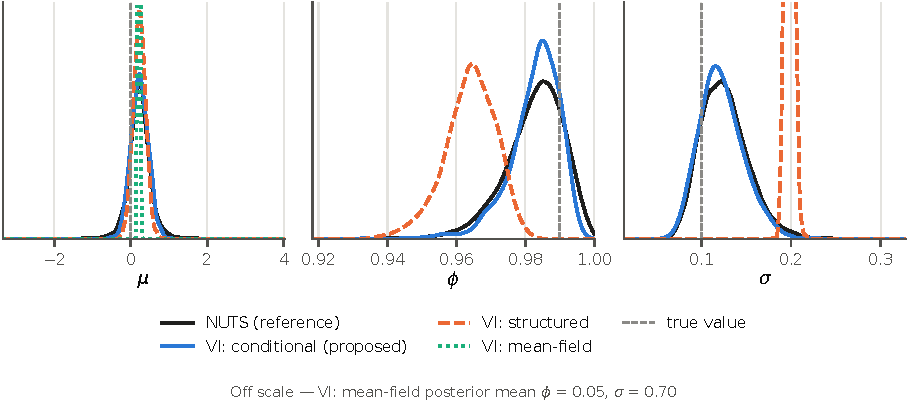
\includegraphics[width=\linewidth]{figures/fig3_theta_marginals.pdf}
  \caption{パラメータの周辺事後分布（S2、高持続シナリオ、$T = 1{,}000$）。
    黒の実線が NUTS（正解）、青の実線が提案手法、橙の破線が構造化、緑の点線が平均場。灰色の縦の破線は真値。
    平均場は $\phi$・$\sigma$ の事後分布が図の範囲外（$\phi \approx 0.05$、$\sigma \approx 0.70$）にある。}
  \label{fig:theta-marginals}
\end{figure}

\begin{figure}[tbp]
  \centering
  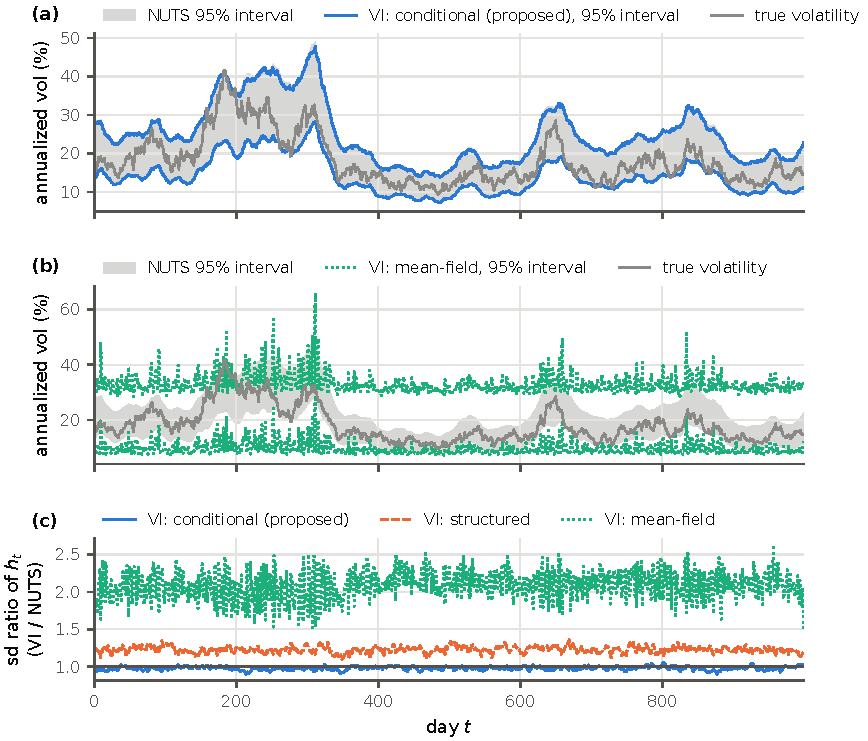
\includegraphics[width=\linewidth]{figures/fig2_h_bands.pdf}
  \caption{潜在ボラティリティの事後区間（S2、高持続シナリオ、$T = 1{,}000$）。
    (a)・(b)：年率ボラティリティ $\sqrt{252}\, e^{h_t/2}$（\%）の 95\% 事後区間。灰色の帯が NUTS、線が VI の区間の上端と下端、灰色の細線が真のボラティリティ。
    (a) は提案手法、(b) は平均場。
    (c)：$h_t$ の事後標準偏差の NUTS に対する比。1 なら NUTS と同じ広がり。}
  \label{fig:h-bands}
\end{figure}

\subsubsection{条件付き構造化（提案）}

提案手法の事後分布は NUTS とよく一致した。
\begin{itemize}
  \item \textbf{パラメータ}：事後平均は $\phi$ が 0.983（NUTS 0.983）、$\sigma$ が 0.123（NUTS 0.126）である。
    \cref{fig:theta-marginals}でも、$\phi$ と $\sigma$ の周辺事後分布は NUTS とほぼ重なる。
    1 次元 Wasserstein 距離は $\phi$ で 0.001、$\sigma$ で 0.003 で、それぞれの事後標準偏差（0.009、0.027）よりも一桁小さい。
    事後標準偏差の比は $\phi$ で 0.87、$\sigma$ で 0.90 で、区間がやや（1 割ほど）狭い。
  \item \textbf{潜在ボラティリティ}：$h_t$ の事後標準偏差の比は中央値 0.98 で、\cref{fig:h-bands}(c) のとおりほぼすべての時点で 1 に近い。
    \cref{fig:h-bands}(a) では、提案手法の 95\% 区間（青線）は NUTS の区間（灰色の帯）の縁にほぼ重なっている。
    事後平均の差は NUTS の事後標準偏差の 0.03 倍（時点の中央値）しかなく、NUTS と見分けがつかない。
  \item \textbf{弱点}：$\mu$ の事後標準偏差は NUTS の 0.66 倍である。
    S1 と同じく、$\phi$ が 1 に近いときの $\mu$–$\phi$ の非線形の依存を表せないためである。
    \cref{fig:theta-marginals}の $\mu$ の図では、NUTS の分布の裾が提案手法より長い。
\end{itemize}

計算時間は、20,000 ステップを回しきって 7.1 秒、ELBO が収束するまで（3,400 ステップ）なら 3.5 秒である。
NUTS（178 秒）と比べると 25〜50 倍速い。

\subsubsection{構造化}

構造化 VI は、$\phi$ の事後平均が 0.964（NUTS 0.983）、$\sigma$ が 0.198（NUTS 0.126）で、とくに $\sigma$ が大きくずれた。
\cref{fig:theta-marginals}の $\sigma$ の図では、構造化の事後分布は $\sigma \approx 0.2$ に鋭く集中し、NUTS の事後分布とほとんど重ならない。
事後標準偏差の比は 0.17 で、\cref{sec:fam-structured}で導いた予測値 $\sigma / \sqrt{2(T-1)} = 0.198 / \sqrt{1998} \approx 0.0044$ は、実際の値 0.0045 とよく一致する。
$\sigma$ の Wasserstein 距離は 0.073 で、提案手法の 20 倍以上である。

$h_t$ については、事後標準偏差の比が 1.23 と広すぎ（\cref{fig:h-bands}(c) の橙の破線）、事後平均の差も NUTS の事後標準偏差の 0.20 倍ある。
$\sigma$ が過大なために、推定されたボラティリティの経路が必要以上に細かく上下していることが原因である。
S1 で見たとおり、構造化 VI の $h_t$ の RMSE は NUTS に近いので、ボラティリティの推定値だけを使う用途では大きな問題にはならないが、
パラメータの不確実性を使う用途（予測分布の幅など）には向かない。

\subsubsection{平均場・低ランク・フルランク}

自前の平均場と NumPyro の平均場（\code{AutoNormal}）は、ともに $\phi \approx 0.05$、$\sigma \approx 0.70$ に崩れた。
\cref{fig:h-bands}(b) では、平均場の 95\% 区間（緑の点線）は日ごとにばらばらに上下し、NUTS の帯から大きく外れている。
上端は年率 30〜40\% 付近、下端は 10\% 付近にほぼ張りついており、ボラティリティの局面の変化をまったく追えていない。
$h_t$ の事後標準偏差は NUTS の約 2 倍（\cref{fig:h-bands}(c)）、事後平均の差は NUTS の事後標準偏差の 1.2 倍である。

パラメータを増やした族も改善しなかった。
ランク 10 の低ランク族（約 12,000 パラメータ）は $\phi = 0.052$、$\sigma = 0.701$ で、平均場とほぼ同じ解に収束した。
フルランク族（約 50 万パラメータ）は 230 秒かけても $\phi = 0.24$、$\sigma = 0.67$ にとどまった。
\cref{fig:elbo}の ELBO の推移を見ると、フルランク族は 20,000 ステップの時点でもまだ ELBO が上昇を続けており、最適化が終わっていない。
\cref{sec:fam-dense}で述べたとおり、パラメータ数を増やすことと、事後分布の構造に合った族を選ぶことは別の問題である。

\subsubsection{ELBO による比較}

\begin{figure}[tbp]
  \centering
  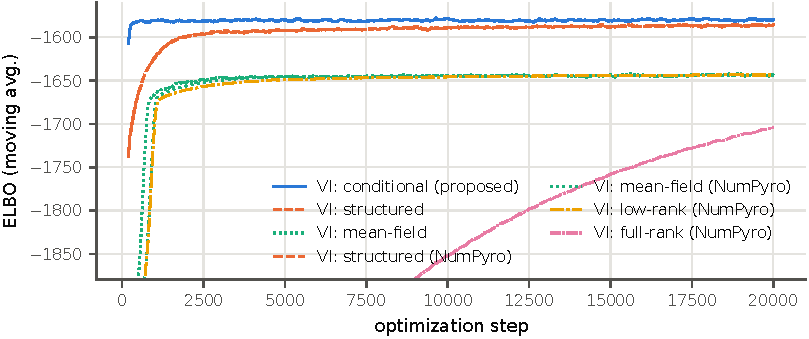
\includegraphics[width=\linewidth]{figures/figA1_elbo.pdf}
  \caption{ELBO の推移（S2、高持続シナリオ、$T = 1{,}000$、200 ステップの移動平均）。
    自前の構造化と NumPyro の構造化の曲線はほぼ重なっている。平均場と低ランクも同じ値に収束する。}
  \label{fig:elbo}
\end{figure}

\cref{fig:elbo}に、最適化中の ELBO の推移を示す。
最終的な ELBO は、提案手法 $-1579.9$、構造化 $-1586.1$、平均場 $-1643.7$、低ランク $-1643.4$、フルランク $-1705.5$ の順である。
ELBO は $\log p(y) - \KL(q \,\|\, p(\cdot \mid y))$ に等しく（\cref{eq:elbo-identity}）、$\log p(y)$ はデータだけで決まって手法によらない。
したがって、ELBO の差はそのまま KL の差であり、提案手法は構造化より約 6 nats、平均場より約 64 nats だけ真の事後分布に近い。
この順位は、パラメータと $h$ の推定の良さの順位と一致している。
同じモデル・同じデータであれば、ELBO を比べることで変分族の良し悪しを判断できる。
これは、実務で変分族や設定を選ぶときの実用的な基準になる（\cref{sec:system}）。

平均場の ELBO が低い値で止まっているのは、最適化が失敗したからではなく、平均場の族の中ではこれが最適だからである。
\cref{tab:meanfield-laplace}で見たように、真の値に近い $\phi$ では平均場近似の KL の最小値が 300 nats を超えるため、
平均場の族の中では、$\log p(y \mid \theta)$ を犠牲にしてでも KL の小さい $\phi \approx 0$ を選ぶ方が ELBO は大きくなる。
平均場の ELBO の曲線は 2,500 ステップほどで平らになっており、最適化そのものは順調に収束している。
「ELBO が収束した」ことは、「事後分布をよく近似できた」ことを意味しないという点は、実務で VI を使ううえで重要な注意点である。

また、自前の構造化と NumPyro の構造化（自作のガイド）は、ELBO（$-1586.1$ と $-1586.3$）・事後平均（$\phi = 0.964$、$\sigma = 0.198$）がともに一致した。
自前の平均場と NumPyro の \code{AutoNormal} も一致している。
独立に書いた二つの実装が同じ結果を出すことは、自前の ADVI の実装の検算になっている。

\subsubsection{PSIS $\hat k$}

$\hat k$ は、提案手法で 0.85、構造化で 1.02、平均場で 1.41、低ランクで 1.25、フルランクで 4.15 であった。
$\hat k$ の大小の順序は近似の良さの順序とおおむね一致するが、提案手法を含むすべての手法で、信頼できる目安とされる 0.7 を超えている。
\cref{sec:inf-diagnostics}で述べたとおり、$\hat k$ は $\theta$ と $h_{1:T}$ をあわせた 1,000 次元を超える同時分布の重要度重みから計算するため、
個々の周辺分布の近似が良くても、高次元での小さなずれが積み重なって大きな値になりやすい。
本稿の結果は、$\hat k$ が「事後分布の同時分布をそのまま重要度サンプリングに使えるか」の基準としては厳しすぎ、
SV モデルの VI の品質の監視には、ELBO の比較や、定期的な NUTS との突き合わせの方が実用的であることを示している（\cref{sec:system}）。

\subsection{計算時間のスケーリング（S3）}\label{sec:syn-scaling}

S3 では、標準シナリオから生成した $T = 250, 500, 1{,}000, 2{,}000, 5{,}000, 10{,}000$ のデータについて、各手法の所要時間を測った。
\cref{fig:scaling}に所要時間を両対数で、\cref{tab:scaling}に数値を示す。
NUTS は 4 連鎖でウォームアップ・サンプリング各 1,000 回の総時間、VI は ELBO が収束するまでの時間である（\cref{sec:syn-setup}）。

\begin{figure}[tbp]
  \centering
  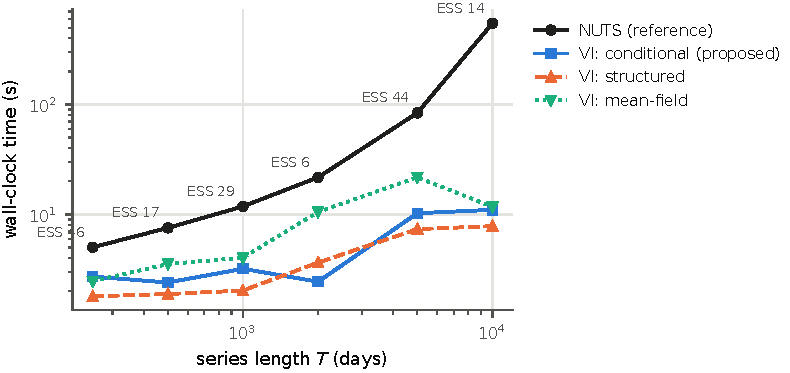
\includegraphics[width=0.88\linewidth]{figures/fig4_scaling.pdf}
  \caption{系列長 $T$ と所要時間（S3、標準シナリオ、両対数）。
    NUTS は 4 連鎖（並列）でウォームアップ・サンプリング各 1,000 回の総時間。VI は ELBO が収束するまでの時間（JIT コンパイルを含む）。
    NUTS の点に添えた数字は、パラメータの最小 ESS（4,000 サンプル中）。}
  \label{fig:scaling}
\end{figure}

\begin{table}[tbp]
  \centering
  \caption{系列長 $T$ と所要時間 [秒]（S3、標準シナリオ）。
    NUTS の時間は総時間、最小 ESS と最大 $\hat R$ はパラメータ $(\mu, \phi, \sigma)$ についての値。
    提案手法は ELBO が収束するまでの時間と、10,000 ステップをすべて実行した総時間の両方を示す。
    ほかの VI は収束するまでの時間。時間はいずれも JIT コンパイルを含む。}
  \label{tab:scaling}
  \small
  \setlength{\tabcolsep}{4pt}
  \begin{tabular}{rrrrrrrrr}
\toprule
 & \multicolumn{3}{c}{NUTS（基準）} & \multicolumn{2}{c}{条件付き構造化（提案）} & \multicolumn{3}{c}{ほかの VI（収束まで）} \\
\cmidrule(lr){2-4} \cmidrule(lr){5-6} \cmidrule(lr){7-9}
$T$ & 時間 & 最小 ESS & 最大 $\hat R$ & 収束まで & 全ステップ & 構造化 & 平均場 & 平均場（NumPyro） \\
\midrule
250 & 5.0 & 46 & 1.04 & 2.7 & 3.0 & 1.8 & 2.5 & 4.2 \\
500 & 7.5 & 17 & 1.53 & 2.4 & 3.0 & 1.9 & 3.5 & 3.7 \\
1,000 & 11.8 & 29 & 1.17 & 3.2 & 4.2 & 2.0 & 4.0 & 8.6 \\
2,000 & 21.7 & 6 & 1.47 & 2.4 & 11.5 & 3.6 & 10.5 & 11.5 \\
5,000 & 83.9 & 44 & 1.04 & 10.3 & 26.0 & 7.4 & 21.8 & 31.1 \\
10,000 & 548.0 & 14 & 1.14 & 11.0 & 52.2 & 7.8 & 11.7 & 29.7 \\
\bottomrule
\end{tabular}

\end{table}

\subsubsection{NUTS}

NUTS の所要時間は、$T = 250$ の 5.0 秒から $T = 10{,}000$ の 548 秒まで、$T$ に比例するよりも速く増えた。
とくに $T = 5{,}000$ から $10{,}000$ では、$T$ が 2 倍になったのに対して時間は 6.5 倍になっている。
NUTS の 1 回の勾配計算は $O(T)$ であるが、次元が大きくなると、事後分布を探索するのに必要なリープフロッグのステップ数（1 回の更新あたりの勾配計算の回数）も増えるためと考えられる。

さらに重要なのは、時間をかけても得られる情報が増えないことである。
パラメータの最小 ESS は、4,000 サンプルに対して 6〜46 しかなく、$T$ によらず小さい（$T = 10{,}000$ で 14）。
$\hat R$ の最大値も 1.04〜1.53 で、6 通り中 4 通りの $T$ で目安の 1.05 を超えている。
つまり、この長さの NUTS の結果は、パラメータについては信頼できる推定とは言えない。
信頼できる結果を得るには、S2 のように連鎖をはるかに長くする必要があり（$T = 1{,}000$ で 178 秒）、所要時間はさらに 1 桁以上増える。
最小 ESS を時間で割った「1 秒あたりの有効サンプル数」は、$T = 250$ の 9.1 から $T = 10{,}000$ の 0.03 まで、約 350 分の 1 に落ちる。

\subsubsection{VI}

提案手法と構造化の VI の所要時間は、$T \le 2{,}000$ では 2〜4 秒でほぼ一定である。
この範囲では、所要時間の大半（約 2 秒）が JIT コンパイルの時間で、最適化そのものは 1 秒程度で終わっている。
$T = 5{,}000$ と $10{,}000$ では、提案手法で約 10〜11 秒になる。
1 ステップの計算量は $O(T)$（\cref{sec:fam-conditional}）なので、10,000 ステップをすべて実行した総時間は $T = 5{,}000$ の 26 秒から $T = 10{,}000$ の 52 秒へと、ほぼ $T$ に比例して増える。
収束までの時間が $T = 5{,}000$ と $10{,}000$ であまり変わらないのは、収束までのステップ数がデータによって 1,800〜3,400 とばらつくためである。

自前実装の平均場と NumPyro の平均場を比べると、NumPyro の方が 1.1〜2.5 倍時間がかかった。
推定結果は同じなので、これは変分族の違いではなく、最適化ループや ELBO の推定のまとめ方といった実装の違いによるものと考えられる。
自前の実装では、最適化のループ全体を一つの関数として JIT コンパイルしている（\cref{sec:system}）。

\subsubsection{速さの比較の読み方}

NUTS と提案手法の速さの比は、どの時間で比べるかによって変わるので、正直に複数の見方を示しておく。

\begin{itemize}
  \item \textbf{収束までの時間で比べる}と、提案手法は $T = 1{,}000$ で約 4 倍、$T = 10{,}000$ で約 50 倍（548 秒に対して 11 秒）速い。
    \cref{sec:intro}の「約 50 倍」はこの比較である。
  \item \textbf{10,000 ステップを回しきった総時間で比べる}と、$T = 1{,}000$ で約 3 倍、$T = 10{,}000$ で約 10 倍（548 秒に対して 52 秒）である。
    収束の判定で自動的に止める実装にすれば前者に、決め打ちのステップ数で回すなら後者に近くなる。
    なお $T = 2{,}000$ では、収束の判定が 800 ステップと早く出ており、収束までの時間（2.4 秒）は総時間（11.5 秒）よりかなり短い。
    収束の判定にはこの程度のばらつきがあるため（その理由は\cref{sec:sys-warm}で述べる）、\cref{fig:scaling}の VI の線の細かい上下は傾向として読むべきである。
  \item \textbf{信頼できる NUTS と比べる}と、差はさらに大きい。
    S3 の NUTS は $\hat R$ が目安を超えており、信頼できる推定には S2 のような長い連鎖が必要になる。
    $T = 1{,}000$ では、S2 の NUTS（178 秒）と提案手法（収束まで 3.5 秒、総時間 7.1 秒）の比は 25〜50 倍である。
\end{itemize}

実データの長さ（$T \approx 480$）で 1 系列だけを推定するなら、NUTS でも数秒〜数十秒で終わり、速さの差は実務上の決め手にならないかもしれない。
VI の速さが効いてくるのは、(i) 系列が長いとき、(ii) 多数の銘柄を一度に推定するとき、(iii) 毎日の再推定のように推定を何度も繰り返すとき、である。
(ii)・(iii) については、実データで\cref{sec:empirical,sec:system}で調べる。

\subsection{設定への感度（S4）}\label{sec:syn-sensitivity}

S4 では、高持続シナリオ（$T = 1{,}000$）のデータ 5 本について、推定の設定を変えたときの結果を比べた。
評価は、各データについて同じ事前分布で回した NUTS（ウォームアップ・サンプリング各 2,000 回）との比で行う。
\cref{tab:sensitivity}に結果を示す。

\begin{table}[tbp]
  \centering
  \caption{設定への感度（S4、高持続シナリオ、$T = 1{,}000$、5 本）。
    $\bar\phi$・$\bar\sigma$ は事後平均の 5 本の平均（真値は 0.99・0.10）、sd 比は NUTS に対する事後標準偏差の比の中央値、
    $h$ の RMSE は真値に対する値の平均、収束 step は ELBO が収束したステップの中央値。
    「中心化」「MC=4」「lr=0.01」は同じ標準の設定を別の乱数で回したものである。}
  \label{tab:sensitivity}
  \footnotesize
  \setlength{\tabcolsep}{3.5pt}
  \begin{tabular}{llrrrrrrr}
\toprule
比較 & 設定 & $\bar\phi$ & $\bar\sigma$ & $\mathrm{sd}(\phi)$比 & $\mathrm{sd}(\sigma)$比 & $\mathrm{sd}(h)$比 & $h$ RMSE & 収束step \\
\midrule
パラメータ化 & meanfield/中心化 & 0.041 & 0.536 & 2.38 & 0.35 & 1.62 & 0.529 & 2600 \\
 & meanfield/非中心化 & 0.039 & 0.555 & 2.32 & 1.35 & 1.70 & 0.528 & 5600 \\
 & structured/中心化 & 0.949 & 0.204 & 0.66 & 0.14 & 1.22 & 0.312 & 3200 \\
 & structured/非中心化 & 0.941 & 0.205 & 0.80 & 0.47 & 1.24 & 0.318 & 2600 \\
 & conditional/中心化 & 0.975 & 0.130 & 0.90 & 0.93 & 0.97 & 0.286 & 1600 \\
 & conditional/非中心化 & 0.975 & 0.129 & 0.90 & 0.87 & 0.97 & 0.285 & 800 \\
\addlinespace
σ の事前分布 & conditional/InvGamma & 0.979 & 0.117 & 0.80 & 0.83 & 0.97 & 0.283 & 1600 \\
\addlinespace
MC サンプル数 & conditional/MC=1 & 0.976 & 0.125 & 0.82 & 0.85 & 0.95 & 0.284 & 5600 \\
 & conditional/MC=4 & 0.975 & 0.129 & 0.92 & 0.92 & 0.98 & 0.285 & 3000 \\
 & conditional/MC=16 & 0.974 & 0.131 & 0.91 & 0.92 & 0.98 & 0.285 & 1800 \\
\addlinespace
学習率 & conditional/lr=0.003 & 0.978 & 0.120 & 0.73 & 0.77 & 0.94 & 0.283 & 2800 \\
 & conditional/lr=0.01 & 0.975 & 0.129 & 0.86 & 0.88 & 0.97 & 0.285 & 2400 \\
 & conditional/lr=0.03 & 0.974 & 0.132 & 0.87 & 0.94 & 0.98 & 0.285 & 1000 \\
\bottomrule
\end{tabular}

\end{table}

\subsubsection{評価そのもののばらつき}

まず、表の数値の読み方として、評価そのもののばらつきの大きさを確かめておく。
表の「条件付き構造化／中心化」「MC=4」「lr=0.01」の 3 行は、いずれも標準の設定（中心化、MC サンプル数 4、学習率 0.01）であり、違うのは最適化の乱数だけである。
この 3 行の間でも、$\sigma$ の sd 比は 0.88〜0.93、$\phi$ の sd 比は 0.86〜0.92、収束ステップは 1,600〜3,000 と変わる。
つまり、sd 比で $\pm 0.05$ 程度、収束ステップで 2 倍程度の違いは、設定の効果ではなく乱数によるばらつきの範囲である。

\subsubsection{パラメータ化}

提案手法は、中心化と非中心化でほぼ同じ結果になった（$\bar\phi = 0.975$ と $0.975$、$\bar\sigma = 0.130$ と $0.129$、$h$ の sd 比はともに 0.97）。
$\sigma$ の sd 比（0.93 と 0.87）の違いは、上のばらつきの範囲に収まる。
これは、\cref{sec:fam-conditional}で示した「提案族はパラメータ化によらず同じ分布の集合になる」という性質を、実験で確かめたものである。
パラメータ化を選ぶ手間（\cref{sec:model-param}）がなくなることは、実務上の利点である。

平均場は、非中心化にしても $\phi \approx 0.04$ に崩れたままであった。
$\sigma$ の sd 比は 0.35 から 1.35 に変わるが、$\phi$ が崩れていることに変わりはない。
平均場の失敗はパラメータ化の問題ではなく、$h_t$ の時間方向の相関を表せないことによる（\cref{sec:inf-vi}）ことが確認できる。

構造化は、非中心化にすると $\sigma$ の sd 比が 0.14 から 0.47 に改善した。
非中心化では $h_t = \mu + \sigma x_t$ と表すので、$q(x)$ が $\theta$ に依存しなくても、$h$ の経路の振れ幅は $\sigma$ に比例して変わる。
つまり、$\sigma$ と $h$ の依存の一部（振れ幅の方向）が、パラメータ化を通じて表されるようになる。
それでも $\sigma$ の sd 比は 0.47 にとどまり、$\bar\sigma$ も 0.205 と過大なままで、提案手法には及ばない。
構造化族では、パラメータ化の選び方で結果が変わり、しかもどちらでも十分ではない。

\subsubsection{$\sigma$ の事前分布}

$\sigma$ の事前分布を、標準の $\mathrm{HalfNormal}(1)$ から、$\sigma^2 \sim \mathrm{InvGamma}(2.5, 0.025)$（事前平均 0.12、95\% 区間 0.06〜0.25。\cref{tab:priors}）に変えると、
提案手法の $\bar\sigma$ は 0.130 から 0.117 に下がり、真値 0.10 に少し近づいた。
これは事前分布が小さい $\sigma$ に情報を持っているためで、NUTS でも同じ方向に動く。
NUTS（同じ事前分布）に対する sd 比は $\phi$ で 0.80、$\sigma$ で 0.83、$h$ で 0.97 で、標準の事前分布のときと大きくは変わらない。
提案手法の近似の質は、事前分布の選び方にはあまり左右されない。

\subsubsection{MC サンプル数と学習率}

ELBO の勾配の MC サンプル数を 1・4・16 と変えても、提案手法の $\bar\phi$（0.974〜0.976）と $\bar\sigma$（0.125〜0.131）はほとんど変わらなかった。
MC サンプル数 1 では sd 比がやや小さく（$\sigma$ で 0.85）、収束ステップが 5,600 と多い。
勾配の雑音が大きいと、最適化に時間がかかり、最終的な変分分布もわずかに狭くなる傾向がある。
1 ステップの計算量は MC サンプル数にほぼ比例するので、本稿の標準の 4 は、精度と計算時間の妥当な折り合いである。

学習率を 0.003・0.01・0.03 と変えた場合も、$\bar\phi$ と $\bar\sigma$ の変化は小さい。
ただし学習率 0.003 では sd 比が $\phi$ で 0.73、$\sigma$ で 0.77 と小さめになった。
学習率が小さいと、10,000 ステップの間に変分分布の広がりの最適化が終わりきらないためと考えられる。
学習率 0.03 では収束が速く（1,000 ステップ）、結果も標準の設定と変わらなかった。
実務で計算時間を短くしたい場合には、学習率を大きめにして早めに打ち切るという選択肢もある。

以上から、提案手法は、パラメータ化・事前分布・最適化の設定のいずれに対しても頑健であり、
設定を細かく調整しなくても安定した結果が得られる。
これは、多数の銘柄を同じ設定で一括して推定する運用（\cref{sec:system}）にとって重要な性質である。

\subsection{まとめ}\label{sec:syn-summary}

本章の合成データ実験の結果をまとめる。

\begin{enumerate}
  \item \textbf{平均場 VI は SV モデルには使えない}。
    持続性 $\phi$ を、真値 0.80〜0.99 に対して 0.03〜0.09 程度（複製の平均）に崩し、$\sigma$ も大きく過大になる。
    データを増やしても、パラメータ化を変えても改善しない。
    低ランク・フルランクの族も同様に崩れる。
    事後分散の過小評価という一般的な問題以前に、点推定そのものが大きく偏る。
  \item \textbf{構造化 VI は $h$ の推定は良いが、$\sigma$ の不確実性を失う}。
    $\sigma$ の 95\% 区間の被覆率は全条件で 0、事後標準偏差は NUTS の 0.07〜0.19 倍で、$\sigma$ の点推定も偏る（偏りの向きはシナリオによって変わる）。
    $\theta$ と $h$ の事後的な依存を表せないことによる。
  \item \textbf{条件付き構造化 VI（提案）は NUTS とほぼ同等の精度を持つ}。
    $\phi$・$\sigma$・$h_t$ の RMSE は NUTS と同程度、$\sigma$ と $h_t$ の区間は名目どおりの被覆率を持ち、
    NUTS の事後分布との比較でも、$h_t$ の事後標準偏差の比は 0.98、事後平均の差は NUTS の事後標準偏差の 0.03 倍である。
    弱点は、$\phi$ の区間がやや（1 割ほど）狭いこと、$\mu$ の不確実性を過小評価すること、レバレッジ SV の $\rho$ を約 25\% 0 の側に縮めることである。
  \item \textbf{提案手法は速い}。
    ELBO の収束までの時間で比べて、$T = 10{,}000$ で NUTS の約 50 倍速く、所要時間は $T$ にほぼ比例して増える。
    NUTS は $T$ とともに時間が超線形に増えるうえ、短い連鎖ではパラメータの混合も不十分である。
    一方、実データの長さ（$T \approx 500$）で 1 系列だけを推定する場合、速さの差は数倍にとどまる。
  \item \textbf{提案手法は設定に頑健である}。
    中心化・非中心化で同じ結果になり、事前分布・MC サンプル数・学習率を変えても結果はほとんど変わらない。
  \item \textbf{ELBO は変分族の良し悪しの比較に使えるが、$\hat k$ は厳しすぎる}。
    同じデータでの ELBO の順位は近似の質の順位と一致した。
    一方、$\hat k$ は提案手法でも 0.85 で、SV モデルの VI の品質監視の主な指標には向かない。
\end{enumerate}

次の\cref{sec:empirical}では、これらの結果が実データでも成り立つかを、日本株の ETF と個別銘柄のデータで確かめる。
とくに、合成データでは確かめられない、モデルの誤特定がある場合の挙動と、VaR の予測という実務上の目的に対する性能を調べる。

% 6 章：R1〜R2（ETF のボラ推定、VaR バックテスト）
\section{実データ分析}\label{sec:empirical}

（執筆予定）

% 7 章：warm start、多銘柄の並列化、収束判定と監視、MCMC との使い分け
\section{システム実装上の考察}\label{sec:system}

（執筆予定）

% 8 章
\section{結論と今後の課題}\label{sec:conclusion}

（執筆予定）


\printbibliography[title={参考文献}]

\appendix
% 付録 A〜D
\section{ELBO の勾配と条件付き構造化変分族の導出}\label{app:derivation}

（執筆予定）

\section{実装の抜粋}\label{app:code}

（執筆予定）

\section{実験設定と感度分析}\label{app:settings}

（執筆予定）

\section{データの取得と前処理}\label{app:data}

（執筆予定）


\end{document}
